\documentclass{article}

\usepackage[a4paper]{geometry}
\usepackage{float}
\usepackage{etoolbox}
\AtBeginEnvironment{tabular}{\small}
\emergencystretch=3em
\usepackage{hyperref}

\usepackage{tikz}
\usetikzlibrary{positioning}
\usepackage{biblatex}
\addbibresource{aotfmt.bib}
\usepackage{minted}
\setminted{breaklines}
\setminted{fontsize=\small}

\title{The Ahead Of Time File Format}
\author{Luca Orlandello}

% "Loader" and "writer" always mean the WAMR-2.4.4 sources below.
\newcommand{\loader}{\texttt{aot\_loader.c}}
\newcommand{\writer}{\texttt{aot\_emit\_aot\_file.c}}

\begin{document}
\maketitle
\tableofcontents

\section{Introduction}
\label{chapter:aot-file-format}
The AOT format is a file format for executables. It is not standard: it is used and developed by the WAMR project \cite{wamr2026}.
The AOT format is designed to make the compilation of a WASM module to machine code easy.
The AOT file format is not officially documented anywhere.
One of the main contributions of this work is the documentation of the AOT file format, done by reverse engineering the open-source WAMR source code (version 2.4.4, git commit \texttt{8c18e3f68b16c4bcaf05996b2636f6ed2b4cf629}).
As this description is based on source code analysis rather than official documentation, some details may be incomplete or imprecise.

The ground truth for this document are two files of the WAMR repository:
\begin{itemize}
    \item the \emph{loader}, \texttt{core/iwasm/aot/aot\_loader.c}, which decides whether a file is accepted by the runtime and how every field is interpreted;
    \item the \emph{writer}, \texttt{core/iwasm/compilation/aot\_emit\_aot\_file.c}, which is the part of the WAMR compiler (\texttt{wamrc}) that serialises an AOT file.
\end{itemize}
When the two disagree, the loader wins, because a file is useful only if the runtime accepts it; the disagreements are pointed out in the text.
Every statement of this document has been checked on files produced by \texttt{wamrc} 2.4.4 for the targets \texttt{x86\_64}, \texttt{i386}, \texttt{aarch64}, \texttt{armv7}, \texttt{thumbv7}, \texttt{mips}, \texttt{riscv32} and \texttt{riscv64}, with and without the XIP and GC options, using the \texttt{readaot} tool described in Appendix~\ref{sec:readaot}.

The description is generic: it covers every architecture and every optional feature supported by WAMR-2.4.4.
Fields that exist only when an optional feature is enabled are marked in the grammars; for example a field marked \texttt{[GC]} is present only when the GC feature flag is set in the target info section (Section~\ref{sec:target-info}).
The parts of the format that depend on the target instruction set (machine code, relocation types) are described in general terms in the main text and per architecture in Appendix~\ref{sec:reloc-arch}.

The AOT file format in this document is specified using a mix of Extended Backus–Naur Form (EBNF) \cite{wikipedia-ebnf} and C struct syntax.
Constraints that cannot be conveniently expressed in EBNF are described in accompanying prose.

\section{WAMR Compiler AOT File Generation}
\label{subsec:how-wasmc-generates-aot}

Before proceeding, it is helpful to understand how the WAMR compiler generates an AOT file, as this context explains many of the design choices in the AOT format.
The WAMR compiler, called \verb|wamrc|, takes a WASM module as input and produces an AOT file as output.
During this process, \verb|wamrc| first compiles the WASM bytecode (i.e., the contents of the code section in the WASM module) into LLVM IR, which is then compiled into a relocatable object file.
On GNU/Linux systems LLVM produces a relocatable ELF object file, whereas for Windows targets it produces a relocatable COFF object file.
The relocatable object file is then combined by \verb|wamrc| with the original WASM module to generate the final AOT file.

Specifically, the target info section, the text section, the relocation section and the object data subsection of the init data section are taken from the relocatable object file, while the rest of the init data section, the function section and the export section are taken from the original WASM module.
As a result, the contents of the target info, text and relocation sections may differ depending on whether an ELF or a COFF relocatable object file is used.

Every WASM function defined by the module (imported functions excluded) becomes a symbol named \texttt{aot\_func\#$n$} in the object file, where $n$ is the index of the function among the \emph{defined} functions (i.e.\ the WASM function index minus the number of imported functions).
When native stack checks are enabled (the default on 32-bit targets), \texttt{aot\_func\#$n$} is a small ``precheck'' wrapper that checks the native stack and then calls the real body, named \texttt{aot\_func\_internal\#$n$}.
These names appear in the relocation section.

The AOT file is therefore a lightweight, pre-linked container: the runtime does not need a general ELF/COFF loader, it only needs to copy the code into executable memory and apply a short list of relocations against a fixed set of symbols.

\medskip
\textbf{Important:} This document describes the AOT files obtained from relocatable \emph{ELF} object files in detail. The differences of COFF (Windows) files are only mentioned where they affect the layout.

\section{Data Representation}
\label{sec:data-representation}

All the integers of the AOT container (section headers, counts, indices, offsets, \dots) are encoded in \textit{little-endian} byte order, \emph{also when the target machine is big-endian}.
This is a consequence of how WAMR is written: the writer stores every integer in host byte order and swaps it to little-endian only when the host running \texttt{wamrc} is big-endian; the loader swaps every integer it reads only when the host running the runtime is big-endian.
Only the opaque payloads (the machine code, the bytes of the object data sections, the data segments) are in the byte order of the target.
A big-endian target is marked by the \verb|bin_type| field of the target info section.

Table~\ref{table:primitive-types} defines the types used throughout this document.

\begin{table}[H]
\centering
\begin{tabular}{ccll}
    \hline
    Type & Size (bytes) & Alignment & Description \\
    \hline
    \verb|u8|  & 1 & 1 & Unsigned 8-bit integer \\
    \verb|u16| & 2 & 2 & Unsigned 16-bit integer \\
    \verb|u32| & 4 & 4 & Unsigned 32-bit integer \\
    \verb|u64| & 8 & 4 & Unsigned 64-bit integer (note: only 4-byte aligned) \\
    \verb|uptr| & 4 or 8 & 4 & \verb|u32| on 32-bit targets, \verb|u64| on 64-bit targets \\
    \verb|String| & $2+n$ & 2 & see below \\
    \hline
\end{tabular}
\caption{Types used in this document.}
\label{table:primitive-types}
\end{table}

The EBNF grammars in this document use these type names as terminals representing the corresponding sequence of bytes in the file.
\verb|i32|, \verb|i64|, \verb|f32| and \verb|f64| are used as aliases of \verb|u32| and \verb|u64| when the bits are a two's complement integer or an IEEE~754 value.
Whether a target is 32-bit or 64-bit is given by the \verb|bin_type| field of the target info section.

\paragraph{Alignment.}
Every multi-byte field has the alignment of Table~\ref{table:primitive-types}, measured from the start of the file.
The loader does not need any explicit padding information: before reading a \verb|u16| it rounds the read position up to a multiple of 2, and before reading a \verb|u32| or a \verb|u64| it rounds it up to a multiple of 4\footnote{This is the \texttt{TEMPLATE\_READ} macro of the loader. The runtime loads the file at a 4-byte aligned address, so aligning the memory address is the same as aligning the file offset.}.
The bytes skipped this way are padding; the writer always fills them with zeros, the loader ignores their value.
For this reason the padding is usually not written in the grammars of this document: every field is implicitly preceded by the padding needed to align it.
Where the writer adds explicit padding that the implicit rule would not produce (for example to 4-byte align a structure that starts with a \verb|u8|), the grammar says so.

A practical consequence is that a \verb|u64| following a \verb|u32| is \emph{not} 8-byte aligned (see the auxiliary data of Section~\ref{section:init-data-auxiliary}).

\paragraph{Strings.}
A \verb|String| is a \verb|u16| length (2-byte aligned) followed by that many bytes.
The length \emph{includes} a terminating zero byte, which must be present: the loader rejects a string whose last byte is not zero, and it uses the string in place, directly in the file buffer.
A length of 0 is accepted and means the empty string\footnote{\texttt{wamrc} never writes it: the empty string is written as length 1 followed by a zero byte.}.
The writer rejects strings whose length, terminating zero included, exceeds 32767 bytes.

\begin{figure}[H]
\begin{minted}{ebnf}
    (* The start of each String must be 2-byte aligned *)
    String =
        u16,   (* n: number of bytes, final zero byte included *)
        { u8 } (* n bytes, the last one is 0x00 *)
        ;
\end{minted}
\caption{Encoding of a string.}
\label{fig:string-grammar}
\end{figure}

\section{AOT File Format and Its Sections}
The AOT file decodes into a file header followed by a sequence of sections, following the grammar shown in Figure~\ref{listing:aot-file-grammar}.
Each section consists of a \verb|u32| section id, a \verb|u32| section size in bytes and the section contents (the \emph{body}).
The section size does not include the 8 bytes of the id and of the size.
The start of each section is 4-byte aligned (by the implicit alignment rule of the \verb|u32| id): between the end of a section and the start of the next one there can be up to 3 padding bytes.
The file may also end with padding bytes.

\begin{figure}[H]
    \begin{minted}{ebnf}
    AOTFile =
        FileHeader,
        TargetInfoSection,
        InitDataSection,
        TextSection,
        FunctionSection,
        ExportSection,
        RelocationSection,
        { CustomSection }
        ;

    Section = u32,  (* section id *)
              u32,  (* body size in bytes *)
              { u8 } (* body *)
              ;
\end{minted}
\caption{The grammar of an AOT file and its sections.}
\label{listing:aot-file-grammar}
\end{figure}

\begin{table}[H]
\centering
\begin{tabular}{lrl}
    \hline
    Name & Id & Section \\
    \hline
    \verb|AOT_SECTION_TYPE_TARGET_INFO| & 0 & Target info, Section~\ref{sec:target-info} \\
    \verb|AOT_SECTION_TYPE_INIT_DATA|   & 1 & Init data, Section~\ref{sec:init-data} \\
    \verb|AOT_SECTION_TYPE_TEXT|        & 2 & Text, Section~\ref{sec:text} \\
    \verb|AOT_SECTION_TYPE_FUNCTION|    & 3 & Function, Section~\ref{sec:function} \\
    \verb|AOT_SECTION_TYPE_EXPORT|      & 4 & Export, Section~\ref{sec:export} \\
    \verb|AOT_SECTION_TYPE_RELOCATION|  & 5 & Relocation, Section~\ref{sec:relocation} \\
    \verb|AOT_SECTION_TYPE_SIGNATURE|   & 6 & Reserved for module signing, rejected by the loader \\
    \verb|AOT_SECTION_TYPE_CUSTOM|      & 100 & Custom, Section~\ref{sec:custom} \\
    \hline
\end{tabular}
\caption{Section ids.}
\label{table:section-ids}
\end{table}

The loader accepts a file only if:
\begin{enumerate}
    \item every section id is one of 0, 1, 2, 3, 4, 5 or 100, and every section fits in the file;
    \item the first section is the target info section;
    \item every other section has the id of the previous section plus one, or it is a custom section.
        As a consequence, once a custom section appears no other required section can follow\footnote{After a custom section the only id allowed besides 100 would be 101, which does not exist.}: custom sections can only be placed at the end of the file, after the relocation section;
    \item the last section is the relocation section or a custom section\footnote{The loader does not check that all the required sections are present when the file ends with a custom section, but a file without some required section is not usable: for example the function pointers would be missing.}.
\end{enumerate}
Each required section appears exactly once, in the order of Figure~\ref{listing:aot-file-grammar}.
All the required sections except the text section must be consumed exactly: the loader rejects a target info, init data, function, export or relocation section with unused bytes at the end.

\section{File Header}

\begin{figure}[H]
\begin{minted}[escapeinside=||]{c}
typedef struct {
        uint8_t    magic[4];
        uint32_t   version;
} FileHeader;
\end{minted}
\caption{AOT file header}
\label{fig:file-header}
\end{figure}

\begin{itemize}
    \item \verb|magic[4]|: A 4 bytes array holding a ``magic number'', identifying the file as an AOT file.
        Read as a little-endian \verb|u32| it is \verb|0x746f6100| (\verb|AOT_MAGIC_NUMBER|).
        \begin{table}[H]
        \centering
        \begin{tabular}{lrl}
            \hline
            Name & Value & Position \\
            \hline
            \verb|MAGIC0| & '\verb|\0|' (0x00) & \verb|magic[0]| \\
            \verb|MAGIC1| & '\verb|a|' (0x61)  & \verb|magic[1]| \\
            \verb|MAGIC2| & '\verb|o|' (0x6f)  & \verb|magic[2]| \\
            \verb|MAGIC3| & '\verb|t|' (0x74)  & \verb|magic[3]| \\
            \hline
        \end{tabular}
        \caption{AOT magic number}
        \end{table}

    \item \verb|version|: This member identifies the AOT file version, the current version is 5 (\verb|AOT_CURRENT_VERSION|).
        The loader accepts only the current version: files of a different version are rejected (``unknown binary version''), there is no backward compatibility.

        \medskip
        \textbf{Important}: This document describes only the AOT file version 5.
\end{itemize}

\section{Target Info Section} \label{sec:target-info}

The target info section has id 0 and is always 48 bytes long. It decodes into the C struct of Figure~\ref{fig:target-info}.

\begin{figure}[H]
\begin{minted}{c}
typedef struct {
        uint16_t   bin_type;      /* offset  0 */
        uint16_t   abi_type;      /* offset  2 */
        uint16_t   e_type;        /* offset  4 */
        uint16_t   e_machine;     /* offset  6 */
        uint32_t   e_version;     /* offset  8 */
        uint32_t   e_flags;       /* offset 12 */
        uint64_t   feature_flags; /* offset 16 */
        uint64_t   reserved;      /* offset 24 */
        char       arch[16];      /* offset 32 */
} TargetInfo;
\end{minted}
\caption{AOT Target Info Section}
\label{fig:target-info}
\end{figure}

\begin{itemize}
    \item \verb|bin_type|:
        This member identifies from which relocatable object file, ELF or COFF, the content of the target info section, text section and relocation section are taken, see Section~\ref{subsec:how-wasmc-generates-aot}.
        This member also identifies whether the AOT file is targeting a 32-bit or 64-bit architecture and whether it is targeting a little-endian or big-endian machine.
        The writer computes it as \verb|LLVMBinaryType - LLVMBinaryTypeELF32L| for ELF files, and sets it explicitly to 4 or 6 for COFF files.

        \begin{table}[H]
        \centering
        \begin{tabular}{lrl}
            \hline
            Name & Value & Meaning \\
            \hline
            \verb|BIN_TYPE_ELF32L| & 0 & ELF,  32-bit, little endian \\
            \verb|BIN_TYPE_ELF32B| & 1 & ELF,  32-bit, big endian \\
            \verb|BIN_TYPE_ELF64L| & 2 & ELF,  64-bit, little endian \\
            \verb|BIN_TYPE_ELF64B| & 3 & ELF,  64-bit, big endian \\
            \verb|BIN_TYPE_COFF32| & 4 & COFF, 32-bit, little endian \\
            \verb|BIN_TYPE_COFF64| & 6 & COFF, 64-bit, little endian \\
            \hline
        \end{tabular}
        \caption{Binary type legal values}
        \label{table:bin-type-legal-value}
        \end{table}

        In Table~\ref{table:bin-type-legal-value} all the little endian entries have the least significant bit set to 0 and all the big endian entries have it set to 1:
        \verb|bin_type & 1| tells whether the target is big endian.
        All the 32-bit entries have the second least significant bit set to 0 and all the 64-bit entries have it set to 1:
        \verb|bin_type & 2| tells whether the target is 64-bit.
        The value 5 is missing for these two reasons.

        The loader only uses these two bits, and rejects the file if they do not match the machine running the runtime (endianness and \verb|sizeof(void *)|).
        The width also decides the size of the \verb|uptr| fields of the function and relocation sections.

    \item \verb|abi_type|:
        This member is never used by WAMR, the WAMR compiler always sets it to 0.

    \item \verb|e_type|:
        Table~\ref{table:e-type-legal-value} contains the possible values for the \verb|e_type| member; the loader rejects any other value.
        \begin{enumerate}
            \item \verb|E_TYPE_REL| means that the target info section, text section and relocation section are taken from a relocatable object file (the \verb|e_type| of the ELF header is copied), see Section~\ref{subsec:how-wasmc-generates-aot}.
            \item \verb|E_TYPE_XIP| has the same meaning of \verb|E_TYPE_REL| but it also enables the WAMR ``execute in place'' mode, see Section~\ref{sec:xip}\footnote{See also \texttt{wasm-micro-runtime/doc/xip.md} in the WAMR repository.}.
                \texttt{wamrc} writes it when it is run with \verb|--xip| or \verb|--enable-indirect-mode|.
        \end{enumerate}

        \begin{table}[H]
        \centering
        \begin{tabular}{lrl}
            \hline
            Name & Value & Meaning \\
            \hline
            \verb|E_TYPE_REL| & 1 & Relocatable object file \\
            \verb|E_TYPE_XIP| & 4 & Relocatable object file, execute in place \\
            \hline
        \end{tabular}
        \caption{e\_type legal values}
        \label{table:e-type-legal-value}
        \end{table}

    \item \verb|e_machine|:
        This member specifies the machine instruction set for which the AOT file is intended, i.e.\ the instruction set of the code in the text section.
        \verb|e_machine| in the AOT target info section has the same meaning and values of \verb|e_machine| in the ELF header \cite[Ch.~2]{elf-spec-gabi-v42} (it is copied from it).
        For COFF files it is the \verb|Machine| field of the COFF header.

        \begin{table}[H]
        \centering
        \begin{tabular}{lrl}
            \hline
            Name & Value & Meaning \\
            \hline
            \verb|E_MACHINE_386|          &      3 & Intel 80386 \\
            \verb|E_MACHINE_MIPS|         &      8 & MIPS \\
            \verb|E_MACHINE_ARM|          &     40 & ARM 32-bit architecture (AArch32), ARM and Thumb \\
            \verb|E_MACHINE_X86_64|       &     62 & AMD x86-64 architecture \\
            \verb|E_MACHINE_ARC_COMPACT|  &     93 & ARC International ARCompact \\
            \verb|E_MACHINE_XTENSA|       &     94 & Tensilica Xtensa Architecture \\
            \verb|E_MACHINE_AARCH64|      &    183 & ARM 64-bit architecture (AArch64) \\
            \verb|E_MACHINE_ARC_COMPACT2| &    195 & Synopsys ARCompact V2 \\
            \verb|E_MACHINE_RISCV|        &    243 & RISC-V 32/64 bit \\
            \verb|E_MACHINE_WIN_I386|     &  0x14c & Windows i386 architecture (COFF) \\
            \verb|E_MACHINE_WIN_X86_64|   & 0x8664 & Windows x86-64 architecture (COFF) \\
            \hline
        \end{tabular}
        \caption{e\_machine values accepted by the loader}
        \label{table:e-machine-legal-values}
        \end{table}

        The difference between \verb|E_MACHINE_X86_64| and \verb|E_MACHINE_WIN_X86_64|, \verb|E_MACHINE_386| and \verb|E_MACHINE_WIN_I386| is due to the difference between the ELF and COFF formats, see Section~\ref{subsec:how-wasmc-generates-aot}.
        \verb|E_MACHINE_X86_64| and \verb|E_MACHINE_386| are taken from the \verb|e_machine| field of an ELF header, while \verb|E_MACHINE_WIN_X86_64| and \verb|E_MACHINE_WIN_I386| have the same meaning of the non Windows version but they are taken from a COFF header.

    \item \verb|e_version|:
        This member identifies the object file version from which the target info section, text section and relocation section are taken, see Section~\ref{subsec:how-wasmc-generates-aot}.
        The loader requires it to be 1.

        \begin{table}[H]
        \centering
        \begin{tabular}{lrl}
            \hline
            Name & Value & Meaning \\
            \hline
             \verb|E_VERSION_CURRENT| & 1 & Current version \\
            \hline
        \end{tabular}
        \caption{e\_version legal values.}
        \label{table:e-version-legal-values}
        \end{table}

    \item \verb|e_flags|:
        This member holds processor-specific flags.
        It is copied from \verb|e_flags| of the ELF header \cite[Ch.~2]{elf-spec-gabi-v42} (0 for COFF files), and its legal values are defined by the ELF processor supplement (psABI) of the instruction set.
        The loader never reads it, so any value is accepted; it is nevertheless useful to describe the code faithfully, because tools such as disassemblers use it.
        For example, for RISC-V \cite[Ch.~8]{riscv-elf-psabi-v1.0} bit 0 (\verb|EF_RISCV_RVC|) says that the code uses compressed instructions and bits 1--2 give the floating point ABI: \texttt{wamrc} targeting \texttt{riscv32} with its default ABI \texttt{ilp32d} writes \verb|0x4| (\verb|EF_RISCV_FLOAT_ABI_DOUBLE|), with \verb|--target-abi=ilp32 --cpu-features=+m,+a,+c| it writes \verb|0x1| (\verb|EF_RISCV_RVC|, soft-float).
        For ARM \texttt{wamrc} writes \verb|0x05000000| (EABI version 5).

    \item \verb|feature_flags|:
        Each bit of this member says that the code in the AOT file uses a WASM feature or a runtime option that the runtime must support.
        Table~\ref{table:feature-flags} lists the bits.
        The loader rejects the file if a bit marked ``checked'' is set and the corresponding feature is disabled in the runtime build; the other bits are not checked, a few of them only select how the runtime builds call stacks.
        \texttt{wamrc} sets a feature bit only if the feature is enabled by its command line \emph{and} actually used by the module, so a WASM 1.0 module normally gets 0.

        \begin{table}[H]
        \centering
        \begin{tabular}{rlll}
            \hline
            Bit & Name & Loader & Meaning \\
            \hline
            0  & \verb|WASM_FEATURE_SIMD_128BIT|        & checked & 128-bit SIMD \\
            1  & \verb|WASM_FEATURE_BULK_MEMORY|        & checked & bulk memory operations \\
            2  & \verb|WASM_FEATURE_MULTI_THREAD|       & checked & threads (thread manager) \\
            3  & \verb|WASM_FEATURE_REF_TYPES|          & checked & reference types \\
            4  & \verb|WASM_FEATURE_GARBAGE_COLLECTION| & checked & GC: \emph{changes the layout} \\
            5  & \verb|WASM_FEATURE_EXCEPTION_HANDLING| & --      & reserved \\
            6  & \verb|WASM_FEATURE_TINY_STACK_FRAME|   & --      & tiny AOT stack frames \\
            7  & \verb|WASM_FEATURE_MULTI_MEMORY|       & --      & reserved \\
            8  & \verb|WASM_FEATURE_DYNAMIC_LINKING|    & --      & reserved \\
            9  & \verb|WASM_FEATURE_COMPONENT_MODEL|    & --      & reserved \\
            10 & \verb|WASM_FEATURE_RELAXED_SIMD|       & --      & reserved \\
            11 & \verb|WASM_FEATURE_FLEXIBLE_VECTORS|   & --      & reserved \\
            12 & \verb|WASM_FEATURE_FRAME_PER_FUNCTION| & --      & AOT frame created once per function \\
            13 & \verb|WASM_FEATURE_FRAME_NO_FUNC_IDX|  & --      & AOT frames without function index \\
            \hline
        \end{tabular}
        \caption{Feature flags.}
        \label{table:feature-flags}
        \end{table}

        \medskip
        \textbf{Important}: Only the GC bit changes the binary layout of the file (types, tables, globals initial values and function section, see the \texttt{[GC]} fields below).
        The other bits only declare what the code needs from the runtime.

    \item \verb|reserved|:
        Reserved for future use, set it to 0. It is not checked by the loader.

    \item \verb|arch[16]|:
        Machine architecture name, a zero terminated string: the loader rejects the file if \verb|arch[15]| is not zero.
        \texttt{wamrc} copies here the target name given with \verb|--target| (e.g.\ \verb|"riscv32"|, \verb|"armv7"|, \verb|"thumbv7em"|), or \verb|"aarch64v8"| for AArch64.
        The remaining bytes between the end of the architecture name and the end of the \verb|arch| buffer must be zero (they are zero in files written by \texttt{wamrc}).

        The architecture name must be consistent with \verb|e_machine|, and with the architecture the runtime is built for.
        The loader checks both with prefix comparisons, as shown in Table~\ref{table:arch-legal-values}:
        first the \verb|arch| string must start with the name associated with \verb|e_machine|, then it must start with the name of the runtime build target.
        For example a \texttt{riscv32} or \texttt{riscv64} file is accepted by every RISC-V runtime of the same width, endianness and features.
        For ARM and AArch64 there is no fixed name: \verb|arch| must start with the build target of the runtime (e.g.\ \verb|"armv7"|, \verb|"thumbv7em"|, \verb|"aarch64v8"|).
        For backward compatibility the loader rewrites \verb|"arm64"| and \verb|"aarch64"| to \verb|"aarch64v8"| before the checks.

        \begin{table}[H]
        \centering
        \begin{tabular}{p{5.4cm}p{6.4cm}}
            \hline
            arch prefix & e\_machine \\
            \hline
            \verb|"x86_64"| & \verb|E_MACHINE_X86_64|, \verb|E_MACHINE_WIN_X86_64| \\
            \verb|"i386"|   & \verb|E_MACHINE_386|, \verb|E_MACHINE_WIN_I386| \\
            runtime build target, e.g.\ \verb|"armv7"|, \verb|"thumbv7"| & \verb|E_MACHINE_ARM| \\
            runtime build target, e.g.\ \verb|"aarch64v8"| & \verb|E_MACHINE_AARCH64| \\
            \verb|"mips"|   & \verb|E_MACHINE_MIPS| \\
            \verb|"xtensa"| & \verb|E_MACHINE_XTENSA| \\
            \verb|"riscv"|  & \verb|E_MACHINE_RISCV|\\
            \verb|"arc"|    & \verb|E_MACHINE_ARC_COMPACT|, \verb|E_MACHINE_ARC_COMPACT2| \\
            \hline
        \end{tabular}
        \caption{arch values.}
        \label{table:arch-legal-values}
        \end{table}

\end{itemize}

\section{Init Data Section}
\label{sec:init-data}
The init data section has id 1.
Its body is a fixed sequence of subsections, without ids or sizes, following the grammar shown in Figure~\ref{fig:init-data-section-grammar}.
Every subsection starts with a \verb|u32| count, so the start of each subsection is 4-byte aligned.

\begin{figure}[H]
\begin{minted}{ebnf}
    InitDataSection =
        InitDataId,
        u32, (* size of the body in bytes *)
        MemorySubsection,
        TableSubsection,
        TypeSubsection,
        ImportGlobalSubsection,
        GlobalSubsection,
        ImportFunctionSubsection,
        AuxiliarySubsection,
        ObjectDataSubsection
        ;
    InitDataId = "0x01", "0x00", "0x00", "0x00" ;
\end{minted}
\caption{Init data section grammar}
\label{fig:init-data-section-grammar}
\end{figure}

The AOT format is designed to make the compilation of a WASM module easy, because many parts of an AOT file can be taken directly from the WASM module with few modifications.
Table~\ref{table:aot-subsection-wasm-section} summarizes from which section of the WASM module the information of each init data subsection is taken.
The main difference with the WASM binary format is that the AOT format does not use LEB128: every integer has a fixed size and alignment, so that the runtime can read it directly.

\begin{table}[H]
\centering
\begin{tabular}{ll}
    \hline
    Init Data Subsection & WASM Sections \\
    \hline
    Memory          & Import, Memory, Data \\
    Table           & Import, Table, Element \\
    Type            & Type \\
    Import Global   & Import \\
    Global          & Global \\
    Import Function & Import \\
    Auxiliary       & Function, Start, Export, Global \\
    Object Data     & - not taken from the WASM module - \\
    \hline
\end{tabular}
\caption{Mapping between init data subsections and WASM sections.}
\label{table:aot-subsection-wasm-section}
\end{table}

\subsection{Value Types}
\label{sec:value-types}
Value types are encoded as a single byte with the same values of the WASM binary format \cite[Secs.~2.3.1 and 5.3.1]{webassembly2019core}.
Table~\ref{table:wasm-value-types} lists them; the reference types and the packed types are used only by the corresponding features.

\begin{table}[H]
\centering
\begin{tabular}{p{3cm}p{6.4cm}p{3.6cm}}
    \hline
    Byte & Value type & Feature \\
    \hline
    \verb|0x7F| & \verb|i32|, 32-bit integer & WASM 1.0 \\
    \verb|0x7E| & \verb|i64|, 64-bit integer & WASM 1.0 \\
    \verb|0x7D| & \verb|f32|, 32-bit floating point & WASM 1.0 \\
    \verb|0x7C| & \verb|f64|, 64-bit floating point & WASM 1.0 \\
    \verb|0x7B| & \verb|v128| & SIMD \\
    \verb|0x70| & \verb|funcref| & tables (WASM 1.0), reference types \\
    \verb|0x6F| & \verb|externref| & reference types \\
    \verb|0x78|, \verb|0x77| & \verb|i8|, \verb|i16| (packed, struct/array fields only) & GC \\
    \verb|0x73|--\verb|0x6A| & abstract heap reference types & GC \\
    \verb|0x64| & \verb|(ref ht)|, followed elsewhere by a heap type & GC, typed function references \\
    \verb|0x63| & \verb|(ref null ht)|, followed elsewhere by a heap type & GC \\
    \verb|0x67|, \verb|0x66|, \verb|0x62|, \verb|0x61| & string references & stringref \\
    \hline
\end{tabular}
\caption{Value types \cite[Secs.~2.3.1 and 5.3.1]{webassembly2019core}.}
\label{table:wasm-value-types}
\end{table}

The types \verb|0x64| and \verb|0x63| need an additional heap type (a type index, or a negative abstract heap type) that does not fit in one byte; WAMR calls them ``multi byte types''.
Where they can appear, the AOT format reserves room for the heap type (see the table, elem segment and type subsections).

\subsection{Initializer Expressions}
\label{sec:init-expr}
Constant expressions of the WASM module (the initial values of globals, the offsets of data and element segments, the elements of element segments, \dots) are encoded as an \verb|InitExpr|, shown in Figure~\ref{fig:init-expr-grammar}.
An \verb|InitExpr| is 4-byte aligned: a \verb|u32| expression type, followed by a payload that depends on the type, as listed in Table~\ref{table:init-expr-type}.
Most of the type values are the WASM opcodes of the corresponding instruction.

\begin{figure}[H]
\begin{minted}{ebnf}
    (* The start of each InitExpr must be 4-byte aligned *)
    InitExpr = u32, (* expression type, Table "Initializer expression types" *)
               InitExprPayload
               ;
    InitExprPayload =
          (* 0x00 none *)
        | u32               (* 0x41 i32.const, 0x43 f32.const (raw bits) *)
        | u64               (* 0x42 i64.const, 0x44 f64.const (raw bits) *)
        | u64, u64          (* 0xFD v128.const: low half, then high half *)
        | u32               (* 0x23 global.get: global index *)
        | u32               (* 0xD2 ref.func: function index, 0xD0 ref.null *)
        | InitExpr, InitExpr (* 0x6A..0x6C, 0x7C..0x7E: binary operator *)
        | GCInitExprPayload (* 0xD3..0xD8: GC only *)
        ;
\end{minted}
\caption{Initializer expression grammar.}
\label{fig:init-expr-grammar}
\end{figure}

\begin{table}[H]
\centering
\begin{tabular}{p{2.1cm}p{3.2cm}p{4.0cm}p{3.3cm}}
    \hline
    Type & Name & Payload & Feature \\
    \hline
    \verb|0x00| & none          & --                           & passive segments, tables \\
    \verb|0x41| & \verb|i32.const| & \verb|u32|                & WASM 1.0 \\
    \verb|0x42| & \verb|i64.const| & \verb|u64|                & WASM 1.0 \\
    \verb|0x43| & \verb|f32.const| & \verb|u32| (IEEE bits)    & WASM 1.0 \\
    \verb|0x44| & \verb|f64.const| & \verb|u64| (IEEE bits)    & WASM 1.0 \\
    \verb|0x23| & \verb|global.get| & \verb|u32| global index  & WASM 1.0 \\
    \verb|0xFD| & \verb|v128.const| & 2 $\times$ \verb|u64| (16 bytes) & SIMD \\
    \verb|0xD2| & \verb|ref.func| & \verb|u32| function index, \verb|0xFFFFFFFF| = null & elements, reference types \\
    \verb|0xD0| & \verb|ref.null| & \verb|u32| (reference type / heap type) & reference types \\
    \verb|0x6A|, \verb|0x6B|, \verb|0x6C| & \verb|i32.add|, \verb|i32.sub|, \verb|i32.mul| & 2 nested \verb|InitExpr| & extended constant expressions \\
    \verb|0x7C|, \verb|0x7D|, \verb|0x7E| & \verb|i64.add|, \verb|i64.sub|, \verb|i64.mul| & 2 nested \verb|InitExpr| & extended constant expressions \\
    \verb|0xD3| & \verb|struct.new| & see Figure~\ref{fig:gc-init-expr} & GC \\
    \verb|0xD4| & \verb|struct.new_default| & \verb|u32| type index & GC \\
    \verb|0xD5| & \verb|array.new| & see Figure~\ref{fig:gc-init-expr} & GC \\
    \verb|0xD6| & \verb|array.new_default| & see Figure~\ref{fig:gc-init-expr} & GC \\
    \verb|0xD7| & \verb|array.new_fixed| & see Figure~\ref{fig:gc-init-expr} & GC \\
    \verb|0xD8| & \verb|ref.i31| & \verb|u32| & GC \\
    \hline
\end{tabular}
\caption{Initializer expression types.}
\label{table:init-expr-type}
\end{table}

For a binary operator the two operands are complete \verb|InitExpr|, each one 4-byte aligned, written left operand first.

\begin{figure}[H]
\begin{minted}{ebnf}
    GCInitExprPayload =
          (* 0xD3 struct.new *)
          u32,  (* struct type index *)
          u32,  (* field count, must match the struct type *)
          { FieldValue }
        | (* 0xD4 struct.new_default *)
          u32   (* struct type index *)
        | (* 0xD5 array.new, 0xD6 array.new_default, 0xD7 array.new_fixed *)
          u32,  (* element value type *)
          u32,  (* array type index *)
          u32,  (* length *)
          { FieldValue } (* 0xD5: one value, 0xD6: none, 0xD7: length values *)
        | (* 0xD8 ref.i31 *)
          u32
        ;
    (* by size of the field type: 1..4 bytes -> u32,
       8 bytes -> u64, 16 bytes (v128) -> 16 bytes;
       references have the size of a target pointer *)
    FieldValue = u32 | u64 | u64, u64 ;
\end{minted}
\caption{GC initializer expression payloads.}
\label{fig:gc-init-expr}
\end{figure}

\subsection{Memory Subsection}
\label{sec:memory-subsection}

The content and the structure of the memory subsection are very similar to the memory and data sections of a WASM module \cite[Secs.~5.5.8 and 5.5.14]{webassembly2019core}.
The memory subsection decodes into a count of imported memories, a vector of memories and a vector of data segments, following the grammar shown in Figure~\ref{fig:memory-subsection-grammar}.

\begin{figure}[H]
\begin{minted}{ebnf}
    MemorySubsection =
        u32, (* import memory count: always 0 *)
        u32, (* number of WASMMemory elements *)
        { WASMMemory },
        u32, (* number of WASMDataSegment elements *)
        { WASMDataSegment }
        ;

    WASMMemory =
        u32, (* flags *)
        u32, (* bytes per page *)
        u32, (* initial page count *)
        u32  (* maximum page count *)
        ;

    (* The start of each WASMDataSegment must be 4-byte aligned *)
    WASMDataSegment =
        u32,      (* is passive: 0 active, 1 passive *)
        u32,      (* memory index *)
        InitExpr, (* offset in the linear memory *)
        u32,      (* n: number of bytes *)
        { u8 }    (* n bytes *)
        ;
\end{minted}
\caption{Memory subsection grammar.}
\label{fig:memory-subsection-grammar}
\end{figure}

\paragraph{Imported memories.}
The first \verb|u32| is the number of imported memories.
\texttt{wamrc} always writes 0, and the loader reads the value but does not read any imported memory entry after it, so the format of an imported memory is not defined.
An imported memory of the WASM module is instead written as a normal memory in the memory vector: the runtime finds its import name in the WASM import section, which it does not have, so in practice it treats it as a memory defined by the module.

\paragraph{Memories.}
Each memory is composed of four \verb|u32| members:
\begin{enumerate}
    \item \verb|flags|, a bit set (Table~\ref{table:memory-flags}). Bit 0 tells whether a maximum page count is present.
    \item The number of bytes in a memory page: 65536 for a normal WASM memory, but it can be changed by the compiler, see Section~\ref{sec:memory-shrink}.
    \item The initial number of memory pages. It must be less than or equal to the maximum number of pages.
    \item The maximum number of memory pages. If bit 0 of the flags is 0 the maximum is not declared; \texttt{wamrc} then writes 65536 (the WASM limit for 32-bit memories). A declared maximum larger than 65536 is also reduced to 65536.
\end{enumerate}

\begin{table}[H]
\centering
\begin{tabular}{rll}
    \hline
    Bit & Name & Meaning \\
    \hline
    0 & \verb|MAX_PAGE_COUNT_FLAG| & the maximum page count is declared \\
    1 & \verb|SHARED_MEMORY_FLAG| & shared memory (threads); requires bit 0 \\
    2 & \verb|MEMORY64_FLAG| & 64-bit memory (memory64 proposal) \\
    \hline
\end{tabular}
\caption{Memory flags. The loader rejects values above 7, a shared memory without maximum, and the bits 1 and 2 when the runtime is built without shared memory or memory64 support.}
\label{table:memory-flags}
\end{table}

WASM 1.0 allows at most one memory.
If the WASM module has no memory, \texttt{wamrc} still writes one memory, with the members: 0, 65536, 0, 0 (flags 0, bytes per page 65536, no pages).

\paragraph{Data segments.}
A data segment initializes a range of a linear memory with a static buffer of bytes \cite[Sec.~5.5.14]{webassembly2019core}.
A data segment is 4-byte aligned and is composed of five members in the following order:
\begin{enumerate}
    \item \verb|is_passive|: 1 for a passive segment (used only by \verb|memory.init|), 0 for an active segment.
    \item The memory index of the memory initialized by an active segment.
    \item The offset of an active segment in the linear memory, an \verb|InitExpr| (Section~\ref{sec:init-expr}): normally \verb|i32.const| (\verb|0x41|), but also \verb|global.get| (\verb|0x23|) of an imported immutable global, \verb|i64.const| (\verb|0x42|) for a 64-bit memory, or an extended constant expression.
        Passive segments have the type \verb|0x00| (none) and no payload.
    \item The number of bytes of the buffer.
    \item The buffer of bytes. The runtime uses it in place, without copying it.
\end{enumerate}
The first two members are meaningful only when the module uses bulk memory operations (feature bit 1): without it \texttt{wamrc} writes two zeros as placeholders (all segments are then active and use memory 0), and a runtime built without bulk memory support ignores them.

The initial contents of a WASM memory are zero-valued bytes, so a compiler can omit data segments made only of zeros.
If a WASM module has been successfully validated and has no WASM memory, it cannot have WASM data segments.

\subsection{Memory Shrink Optimization}
\label{sec:memory-shrink}

The members of the memory written by \texttt{wamrc} are not always the ones declared by the WASM module.
The WAMR WASM loader, which \texttt{wamrc} uses to parse the module, rewrites the first memory (imported or defined) when the module contains no \verb|memory.grow| and no \verb|memory.size| instruction in any function, in two steps:

\begin{figure}[H]
\begin{minted}{python}
# Step 1 (WASM_ENABLE_SHRUNK_MEMORY, enabled in wamrc):
# only when __data_end, __heap_base and the stack pointer
# global were all found (Section "Auxiliary Subsection")
shrunk = align_up(heap_base, 8)
if shrunk <= bytes_per_page * initial_page_count:
    bytes_per_page = shrunk
    initial_page_count = 1

# Step 2 (always, wamrc is built without multi-module support):
if initial_page_count < 65536:
    bytes_per_page *= initial_page_count
    if initial_page_count > 0:
        initial_page_count = maximum_page_count = 1
    else:
        initial_page_count = maximum_page_count = 0
\end{minted}
\caption{Memory shrink optimization performed by \texttt{wamrc}.}
\label{fig:memory-shrink-optimization}
\end{figure}

Typically, a WASM module compiled from C has a memory of two or more pages of 64~KiB each, so the runtime must allocate a contiguous array of at least 128~KiB for the linear memory.
On devices with very limited memory, external fragmentation may prevent the allocation of such a region.
With the transformation of Figure~\ref{fig:memory-shrink-optimization} the runtime allocates a single ``page'' that is just large enough for the data and the stack (see Section~\ref{section:init-data-auxiliary} and Figure~\ref{fig:linear-memory-layout}), and the module cannot grow its memory anyway because it contains no \verb|memory.grow|.
If the WASM module calls \verb|malloc|, the call can be served by the heap of the WAMR runtime rather than by the part of the linear memory dedicated to the heap.

This is a policy of \texttt{wamrc}, not a requirement of the format: a compiler can write the memory exactly as declared by the WASM module.
The bytes per page value is used by the runtime to compute the memory size and by \verb|memory.size|/\verb|memory.grow|, so changing it is only safe when those instructions are absent.

\subsection{Table Subsection}
\label{sec:table-subsection}

The content and structure of the table subsection are very similar to the table, import and element sections of a WASM module \cite[Secs.~5.5.5, 5.5.7 and 5.5.12]{webassembly2019core}.
The table subsection decodes into a vector of imported tables, a vector of tables and a vector of element segments (called ``table init data'' in WAMR), as defined by the grammar in Figure~\ref{fig:table-subsection-grammar}.
Note that there are always three counts: a module without tables writes three zero \verb|u32|.

\begin{figure}[H]
\begin{minted}{ebnf}
    TableSubsection =
        u32, (* number of WASMImportTable elements *)
        { WASMImportTable },
        u32, (* number of WASMTable elements *)
        { WASMTable },
        u32, (* number of WASMElemSegment elements *)
        { WASMElemSegment }
        ;

    WASMImportTable = TableType ;
    WASMTable = TableType, [ InitExpr ] (* [GC]: initial value *) ;

    TableType =
        u8,   (* element value type *)
        u8,   (* flags *)
        u8,   (* possible grow: 0 or 1 *)
        u8,   (* [GC] nullable of the element ref type, else padding 0 *)
        u32,  (* initial size *)
        u32,  (* maximum size *)
        [ u32 ] (* [GC] heap type, only if the element type is 0x63/0x64 *)
        ;

    (* The start of each WASMElemSegment must be 4-byte aligned *)
    WASMElemSegment =
        u32,      (* mode: WASM element segment flags, 0..7 *)
        u32,      (* element value type *)
        u32,      (* table index *)
        InitExpr, (* offset in the table, type 0x00 if not active *)
        u16,      (* [GC] ref type, else the element type *)
        u16,      (* [GC] nullable, else 0 *)
        u32,      (* [GC] heap type, else 0 *)
        u32,      (* n: number of elements *)
        { InitExpr } (* n elements *)
        ;
\end{minted}
\caption{Grammar of the table subsection.}
\label{fig:table-subsection-grammar}
\end{figure}

\paragraph{Tables.}
The imported tables come first, in the order of the WASM import section, then the tables defined by the module; the table index space of the module is the concatenation of the two vectors.
The import module and field names of imported tables are not written in the file\footnote{The writer has a \texttt{TODO} for them.}.
The members of a table type are:
\begin{itemize}
    \item the element type: \verb|0x70| (\verb|funcref|), \verb|0x6F| (\verb|externref|), or a GC reference type;
    \item the flags: bit 0 tells whether the maximum size is declared, bit 1 means shared (not supported: the loader only records an error message, without rejecting the file), bit 2 is a 64-bit table (memory64 proposal); the loader rejects values above 5 for the defined tables, and does not check the imported ones;
    \item \verb|possible_grow|: 1 if the module contains a \verb|table.grow| instruction for the table, 0 otherwise;
    \item one byte that is the \verb|nullable| flag of the element reference type in GC mode, and a zero padding byte otherwise;
    \item the initial and the maximum size, in elements. \texttt{wamrc} limits the maximum size to $d = \max(2 \times \mathit{initial}, 1024)$: when no maximum is declared it writes $d$, otherwise $\min(\mathit{maximum}, d)$ (or the maximum unchanged if it equals the initial size).
\end{itemize}
In GC mode a table whose element type is \verb|0x63| or \verb|0x64| is followed by the \verb|u32| heap type, and every defined table (not the imported ones) is followed by an \verb|InitExpr| with its initial value (type \verb|0x00| when the table has no initializer).

\paragraph{Element segments.}
Element segments initialize ranges of tables with function references \cite[Sec.~5.5.12]{webassembly2019core}.
\begin{itemize}
    \item \verb|mode| is the flags field of the WASM element segment, between 0 and 7: bit 0 set means passive or declarative, bits 0 and 1 both set mean declarative, otherwise the segment is active.
    \item The element value type, as a \verb|u32|. For a WASM 1.0 segment (mode 0) WAMR uses \verb|0x64| (a non-nullable function reference); explicit \verb|funcref| element kinds give \verb|0x70|.
    \item The index of the table initialized by an active segment.
    \item The offset of an active segment in the table, an \verb|InitExpr| (type \verb|0x00| for passive and declarative segments).
    \item Eight bytes describing the element reference type in GC mode (\verb|u16| reference type, \verb|u16| nullable flag, \verb|u32| heap type), present only if the element type is \verb|0x63| or \verb|0x64|.
        Without GC they are always present and ignored by the loader; \texttt{wamrc} writes the element type, 0 and 0.
    \item The number of elements, then each element as an \verb|InitExpr|: \verb|ref.func| (\verb|0xD2|) with the function index (in the index space that includes the imported functions), \verb|ref.null| (\verb|0xD0|), or with GC any constant expression.
\end{itemize}

\subsection{Type Subsection}

The content and structure of the type subsection are very similar to the type section of a WASM module \cite[Sec.~5.5.4]{webassembly2019core}.
The type subsection decodes into a vector of types following the grammar shown in Figure~\ref{fig:type-subsection-grammar}.
The start of each type is 4-byte aligned.
Without GC every type is a function type, composed of four members:
\begin{itemize}
    \item \verb|TypeFlag|: a \verb|u16| that is 0 (\verb|WASM_TYPE_FUNC|).
        The non-GC loader does not check it; in GC mode it distinguishes the type kinds.
    \item A \verb|u16| with the number of parameters of the function type.
    \item A \verb|u16| with the number of results of the function type.
    \item An array of value types (Section~\ref{sec:value-types}) whose length is the sum of the number of parameters and the number of results: first the types of the parameters, then the types of the results.
\end{itemize}
The loader checks that every value type is valid, and that the parameters and the results do not need more than 65535 cells (Section~\ref{sec:function}).

\begin{figure}[H]
\begin{minted}{ebnf}
    TypeSubsection =
        u32, (* number of WASMType elements *)
        { WASMType }
        ;

    (* without GC; the start of each WASMType must be 4-byte aligned *)
    WASMType =
        TypeFlag,
        u16, (* number of parameters *)
        u16, (* number of results *)
        { WASMValtype } (* parameters, then results *)
        ;

    TypeFlag = "0x00", "0x00" ;
\end{minted}
\caption{Grammar of the type subsection (without GC).}
\label{fig:type-subsection-grammar}
\end{figure}

\paragraph{GC types.}
When the GC feature flag is set, every type has the layout of Figure~\ref{fig:gc-type-grammar}.
A type identical to a previous one (WAMR deduplicates equivalent recursive types) is written as a reference to it.
A \emph{reference type map} gives the full reference type of the parameters, results or fields whose value type is \verb|0x63| or \verb|0x64|.

\begin{figure}[H]
\begin{minted}{ebnf}
    (* GC only; the start of each GCType must be 4-byte aligned *)
    GCType =
          u16,  (* type flag: 0 func, 1 struct, 2 array *)
          "0x01", (* equivalent to a previous type *)
          u8,   (* padding *)
          u32   (* index of the equivalent previous type *)
        | u16,  (* type flag *)
          "0x00",
          u8,   (* is_sub_final *)
          u32,  (* parent type index, 0xFFFFFFFF if none *)
          u16,  (* rec_count: size of the recursion group *)
          u16,  (* rec_idx: index in the recursion group *)
          ( FuncType | StructType | ArrayType )
        ;

    FuncType =
        u16, (* number of parameters *)
        u16, (* number of results *)
        u16, (* m: number of reference type maps *)
        { WASMValtype }, (* parameters, then results *)
        (* only if m > 0: padding to 4 bytes *)
        { RefTypeMap }   (* m maps *)
        ;
    StructType =
        u16, (* number of fields *)
        u16, (* m: number of reference type maps *)
        { u8, (* field flags: bit 0 mutable *)
          WASMValtype },
        (* padding to 4 bytes *)
        { RefTypeMap }   (* m maps *)
        ;
    ArrayType =
        u16, (* element flags: bit 0 mutable *)
        WASMValtype,     (* element type *)
        [ u8,            (* nullable, if the element type is 0x63/0x64 *)
          u32 ]          (* heap type, if the element type is 0x63/0x64 *)
        ;
    RefTypeMap =
        u16, (* index of the parameter/result/field *)
        u8,  (* reference type *)
        u8,  (* nullable *)
        u32  (* heap type *)
        ;
\end{minted}
\caption{Grammar of a type in GC mode.}
\label{fig:gc-type-grammar}
\end{figure}

\subsection{Import Global Subsection}
The content and structure of the import global subsection are very similar to the import section of a WASM module \cite[Sec.~5.5.5]{webassembly2019core}.
The import global subsection decodes into a vector of imported globals, following the grammar shown in Figure~\ref{fig:import-global-subsection-grammar}.
Each imported global is 2-byte aligned and is composed of its value type, a mutability flag (0 immutable, 1 mutable), the import module name and the import field name.
The imported globals take the first indices of the global index space of the module.

\begin{figure}[H]
\begin{minted}{ebnf}
    ImportGlobalSubsection =
        u32, (* number of WASMImportGlobal elements *)
        { WASMImportGlobal }
        ;

    (* The start of each WASMImportGlobal must be 2-byte aligned *)
    WASMImportGlobal =
        WASMValtype,
        IsMutable,
        String, (* module name *)
        String  (* global name *)
        ;
    IsMutable = "0x00" | "0x01" ;
\end{minted}
\caption{Grammar of the import global subsection.}
\label{fig:import-global-subsection-grammar}
\end{figure}

The runtime links the imported globals by name at instantiation; with the built-in libc it resolves some of them while loading and checks that their type and mutability match.

\subsection{Global Subsection}
The content and structure of the global subsection are very similar to the global section of a WASM module~\cite[Sec.~5.5.9]{webassembly2019core}.
The global subsection decodes into a vector of the globals defined by the module, following the grammar shown in Figure~\ref{fig:global-subsection-grammar}.
Each global is 4-byte aligned and consists of three members in the following order:
\begin{enumerate}
    \item A value type (Section~\ref{sec:value-types}).
    \item A one-byte mutability flag.
    \item The initial value, an \verb|InitExpr| (Section~\ref{sec:init-expr}), which is 4-byte aligned: there are always two padding bytes between the mutability flag and the initial value.
        WASM 1.0 allows a constant of the type of the global, or \verb|global.get| of an imported immutable global.
\end{enumerate}
The index of the $i$-th global of this subsection in the global index space is the number of imported globals plus $i$.

\begin{figure}[H]
\begin{minted}{ebnf}
    GlobalSubsection =
        u32, (* number of WASMGlobal elements *)
        { WASMGlobal }
        ;

    (* The start of each WASMGlobal must be 4-byte aligned *)
    WASMGlobal =
        WASMValtype,
        IsMutable,
        (* 2 padding bytes *)
        InitExpr
        ;
\end{minted}
\caption{Global subsection grammar.}
\label{fig:global-subsection-grammar}
\end{figure}

\subsection{Import Function Subsection}
The content and structure of the import function subsection are very similar to the import section of a WASM module~\cite[Sec.~5.5.5]{webassembly2019core}.
The import function subsection decodes into a vector of imported functions following the grammar shown in Figure~\ref{fig:import-function-subsection-grammar}.
Each imported function is composed of a \verb|u16| type index (into the type subsection), the import module name and the import field name.
The imported functions take the first indices of the function index space of the module.

\begin{figure}[H]
\begin{minted}{ebnf}
    ImportFunctionSubsection =
        u32, (* number of WASMImportFunction elements *)
        { WASMImportFunction }
        ;

    WASMImportFunction =
        u16,    (* type index *)
        String, (* module name *)
        String  (* function name *)
        ;
\end{minted}
\caption{Import function subsection grammar.}
\label{fig:import-function-subsection-grammar}
\end{figure}

The runtime resolves the imported functions by name while loading, against the native functions registered by the embedder (or the built-in libc/WASI); a function that cannot be resolved does not prevent loading, and calling it raises the exception ``failed to call unlinked import function''.
The compiled code does not call imported functions directly: it calls them through the runtime function \verb|aot_invoke_native| (Section~\ref{sec:relocation}).

\subsection{Auxiliary Subsection}
\label{section:init-data-auxiliary}

The auxiliary subsection decodes into the tuple of Figure~\ref{fig:auxiliary-subsection-grammar}.
Remember that the \verb|u64| fields are only 4-byte aligned: the whole subsection is 48 bytes long without any padding.

\begin{figure}[H]
\begin{minted}{ebnf}
AuxiliarySubsection =
    u32, (* function count *)
    u32, (* start function index *)
    u32, (* aux data end global index *)
    u64, (* aux data end *)
    u32, (* aux heap base global index *)
    u64, (* aux heap base *)
    u32, (* aux stack top global index *)
    u64, (* aux stack bottom *)
    u32  (* aux stack size *)
    ;
\end{minted}
\caption{Auxiliary subsection grammar}
\label{fig:auxiliary-subsection-grammar}
\end{figure}

\paragraph{Basic fields}

\begin{itemize}
\item Function count: the number of functions \emph{defined} by the module, i.e.\ imported functions excluded. It is also the number of entries of the vectors of the function section.
\item Start function index: the index, in the function index space (imported functions included), of the start function \cite[Sec.~5.5.11]{webassembly2019core}, or \verb|0xFFFFFFFF| if the module has no start function.
    The loader rejects an index out of range. A start function that is an imported function is accepted but not called by WAMR-2.4.4.
\end{itemize}

The remaining fields describe the \textit{layout of the WASM linear memory}.
The runtime uses them to check the native stack of the WASM application (the ``auxiliary stack'') and to share the WASM heap; they are not needed to run the code, and a compiler can always write the default values listed below.
The loader only checks that the three addresses are below 4~GiB.

\paragraph{Linear memory layout}

WASM modules are typically generated by compiling a high-level language rather than being written manually. For example, \verb|clang| can compile a C program into a WASM module.
During this compilation process, the C memory layout (initialized data, uninitialized data, stack, and heap) is mapped onto the WASM linear memory.
Initialized and uninitialized data are mapped in a single data region inside the WASM linear memory.
The linker (\texttt{wasm-ld}) records in the WASM module where the data region ends and where the heap starts, as two exported immutable globals, \verb|__data_end| and \verb|__heap_base|, and keeps the stack pointer in a mutable global (\verb|__stack_pointer|, which is usually not exported).
By default the stack is placed after the data and grows downwards, towards the data.
Figure~\ref{fig:linear-memory-layout} summarizes the resulting linear memory layout.

\begin{figure}[H]
\centering
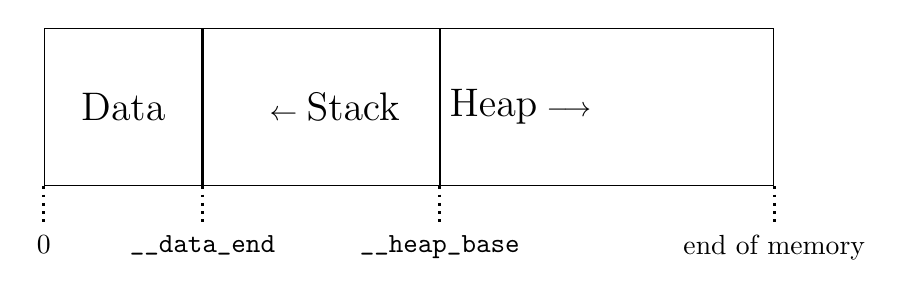
\begin{tikzpicture}[node distance=0]
\node[rectangle, draw=black, minimum width=2cm, minimum height=2cm](data){\Large Data};
\node[rectangle, draw=black, minimum width=3cm, minimum height=2cm, text width=2cm, align=right](stack)[right=of data]{$\leftarrow$ {\Large Stack}};
\node[rectangle, draw=black, minimum width=4cm, minimum height=2cm, text width=4cm, align=left](heap)[right=of stack]{{\Large Heap} $\longrightarrow$ };

\coordinate (dataBottomLeftCorner) at (data.south west);
\coordinate (dataStartLabel) at ([yshift=-0.5cm] dataBottomLeftCorner);

\coordinate (dataBottomRightCorner) at (data.south east);
\coordinate (dataEndLabel) at ([yshift=-0.5cm] dataBottomRightCorner);

\coordinate (stackBottomRightCorner) at (stack.south east);
\coordinate (heapBaseLabel) at ([yshift=-0.5cm] stackBottomRightCorner);

\coordinate (heapBottomRightCorner) at (heap.south east);
\coordinate (maxMemoryLabel) at ([yshift=-0.5cm] heapBottomRightCorner);

\draw[dotted, line width=1pt] (dataBottomLeftCorner) -- (dataStartLabel);
\node[below] at (dataStartLabel) {0};

\draw[dotted, line width=1pt] (dataBottomRightCorner) -- (dataEndLabel);
\node[below] at (dataEndLabel) {\verb|__data_end|};

\draw[dotted, line width=1pt] (stackBottomRightCorner) -- (heapBaseLabel);
\node[below] at (heapBaseLabel) {\verb|__heap_base|};

\draw[dotted, line width=1pt] (heapBottomRightCorner) -- (maxMemoryLabel);
\node[below] at (maxMemoryLabel) {end of memory};

\end{tikzpicture}
\caption{Linear memory layout of a WASM module compiled from a C program.}
\label{fig:linear-memory-layout}
\end{figure}

\paragraph{Default values}

If the layout cannot be detected, the fields are filled with the following default values:

\begin{itemize}
\item aux data end global index: \verb|0xFFFFFFFF|; aux data end: 0;
\item aux heap base global index: \verb|0xFFFFFFFF|; aux heap base: 0;
\item aux stack top global index: \verb|0xFFFFFFFF|; aux stack bottom: 0;
\item aux stack size: 0.
\end{itemize}

\paragraph{Detecting the layout}

\texttt{wamrc} (in fact the WAMR WASM loader it uses) detects the layout with the algorithm of Figure~\ref{figure:aux-detection}.
\verb|__data_end| and \verb|__heap_base| are recognised only if they are exported, defined by the module (not imported), of type \verb|i32|, immutable and initialized with an \verb|i32.const|.

\begin{figure}[H]
\begin{minted}{python}
def detect_aux(module):
    data_end = heap_base = None
    for e in module.exports:            # in export order
        if e.kind != GLOBAL:
            continue
        if e.name in ("__heap_base", "__data_end"):
            if e.index < module.import_global_count:
                continue                 # imported: ignored
            g = module.globals[e.index - module.import_global_count]
            if g.type == I32 and not g.mutable and g.init.type == I32_CONST:
                if e.name == "__heap_base":
                    heap_base = (e.index, g.init.value)
                else:
                    data_end = (e.index, align_up(g.init.value, 16))
        if data_end and heap_base and data_end[1] <= heap_base[1]:
            # the stack pointer: first defined mutable i32 global
            # initialized with an i32.const <= heap base
            for i, g in enumerate(module.globals):
                if (g.mutable and g.type == I32 and g.init.type == I32_CONST
                        and g.init.value <= heap_base[1]):
                    top = g.init.value
                    size = top - data_end[1] if top > data_end[1] else top
                    stack = (module.import_global_count + i, top, size)
                    break
            else:
                stack = (heap_base[0], heap_base[1], 0)
            return data_end, heap_base, stack
    return None   # use the default values
\end{minted}
\caption{Detection of the linear memory layout performed by \texttt{wamrc}.}
\label{figure:aux-detection}
\end{figure}

When the layout is detected, the fields are filled as follows (note that the value of \verb|__data_end| is rounded up to a multiple of 16):
\begin{itemize}
\item aux data end global index and aux data end: the global index of \verb|__data_end| and its initial value rounded up to a multiple of 16;
\item aux heap base global index and aux heap base: the global index of \verb|__heap_base| and its initial value;
\item aux stack top global index: the global index (in the global index space, imported globals included) of the stack pointer global;
\item aux stack bottom: the initial value of the stack pointer, i.e.\ the highest address of the stack, where the stack starts before growing downwards;
\item aux stack size: the initial value of the stack pointer minus the aux data end, or the initial value of the stack pointer if it is not above the aux data end.
\end{itemize}
If no candidate stack pointer global exists, the stack is considered unused: the aux stack top global index and the aux stack bottom are those of \verb|__heap_base| and the aux stack size is 0.

\subsection{Object Data Subsection}
\label{sec:object-data}
The object data subsection contains the data sections of the relocatable object file that the code needs at run time: constants, jump tables and global variables generated by the compiler (not WASM data).
It decodes into a vector of object data sections following the grammar shown in Figure~\ref{fig:object-data-subsection-grammar}.
Each element is composed of the name of the section in the object file, a \verb|u32| size (4-byte aligned) and the section contents.

\begin{figure}[H]
\begin{minted}{ebnf}
    ObjectDataSubsection =
        u32, (* number of ObjectData elements *)
        { ObjectData }
        ;

    ObjectData =
        String, (* section name *)
        u32,    (* n: size in bytes *)
        { u8 }  (* n bytes *)
        ;
\end{minted}
\caption{Object data subsection grammar.}
\label{fig:object-data-subsection-grammar}
\end{figure}

\texttt{wamrc} copies the sections named \verb|.data|, \verb|.sdata|, \verb|.rodata|, \verb|.srodata|, \verb|.rodata.cst*|, \verb|.srodata.cst*|, \verb|.rodata.str*|, \verb|.rdata| (COFF, only if it has relocations), \verb|.aot_stack_sizes| and, with profile guided optimization, \verb|__llvm_prf_*|.
For example on RISC-V the floating point constants of the code are usually in \verb|.sdata| or \verb|.srodata.cst8|.
The section \verb|.aot_stack_sizes| contains one \verb|u32| per defined function, the native stack size the function needs; it is written when native stack checks are enabled and is used by the precheck wrappers (Section~\ref{subsec:how-wasmc-generates-aot}).

The runtime copies every object data section to its own page-aligned memory (or, when possible, right after the code), applies the data relocations (Section~\ref{sec:relocation}) and makes \verb|.rodata*| and \verb|.rdata| read-only.
The code refers to these sections only by their names, through relocations: the names must be unique and must be among those listed above, otherwise the relocations cannot be resolved.

\section{Text Section}
\label{sec:text}
The text section has id 2.
It decodes into a literal pool and the machine code of all the compiled WASM functions, following the grammar shown in Figure~\ref{fig:text-section-grammar}.

\begin{figure}[H]
\begin{minted}{ebnf}
    TextSection =
        TextId,
        u32,    (* size of the body in bytes *)
        u32,    (* l: literal size in bytes *)
        { u8 }, (* l bytes: literal pool *)
        { u8 }  (* the code: all the remaining bytes *)
        ;

    TextId = "0x02", "0x00", "0x00", "0x00" ;
\end{minted}
\caption{Text section grammar.}
\label{fig:text-section-grammar}
\end{figure}

\paragraph{Literal pool.}
The literal pool is the \verb|.literal| section of the object file. It is used only by Xtensa, whose code loads constants and addresses from it with PC-relative \verb|l32r| instructions; for all the other architectures the literal size is 0.
The writer pads the literal pool with zeros to a multiple of 4 bytes, but writes the unpadded size; the loader instead places the code exactly literal size bytes after the end of the size field.
The two agree only if the literal size is a multiple of 4, so a generator must write a literal pool whose size is a multiple of 4.

\paragraph{Code.}
The code is the \verb|.text| section of the object file (\verb|.ltext| with the large code model).
When LLVM splits functions into cold and hot parts, the sections \verb|.text.unlikely.| and \verb|.text.hot.| are appended after \verb|.text|, in this order, each padded to a multiple of 4 bytes; all the offsets of the function and relocation sections refer to the concatenated code.
The code extends to the end of the section: its size is the section size minus 4 minus the literal size.
The text section must not be empty if the module defines functions.

The entry point of each function is given by the function section (Section~\ref{sec:function}).
The code is position independent with respect to everything the runtime provides: every reference to a function, to a data section, to the literal pool or to a runtime function is described by a relocation (Section~\ref{sec:relocation}).

\paragraph{Loading.}
In the normal (non-XIP) mode the runtime copies the whole body of the text section (literal size field and literal pool included) to newly allocated executable memory, enlarged by a \emph{procedure linkage table} (PLT) for the runtime functions (Appendix~\ref{sec:reloc-arch}).
The PLT is created by the runtime and is not part of the file: the size of the PLT depends on the runtime build, and it is included in the code size the runtime uses for the bounds checks.
In XIP mode the code is executed where it is, without copying it and without a PLT.

\section{Function Section}
\label{sec:function}
The function section has id 3.
The content and structure of the function section are very similar to the function section of a WASM module~\cite[Sec.~5.5.6]{webassembly2019core}.
The function section decodes into four vectors, plus a fifth one in GC mode, following the grammar shown in Figure~\ref{fig:function-section-grammar}.
The vectors have no count: each one has as many elements as the function count of the auxiliary subsection (Section~\ref{section:init-data-auxiliary}), i.e.\ one element per defined function.

\begin{figure}[H]
\begin{minted}{ebnf}
    FunctionSection =
        FunctionId,
        u32,      (* size of the body in bytes *)
        { uptr }, (* text offset of each defined function *)
        { u32 },  (* type index of each defined function *)
        { u32 },  (* max local cell number of each defined function *)
        { u32 },  (* max stack cell number of each defined function *)
        [ { LocalRefFlags } ] (* [GC]: one per function, imported included *)
        ;

    FunctionId = "0x03", "0x00", "0x00", "0x00" ;

    LocalRefFlags =
        u32,    (* n: number of cells *)
        { u8 }  (* n flags: 1 if the cell holds a GC reference *)
        ;
\end{minted}
\caption{Function section grammar.}
\label{fig:function-section-grammar}
\end{figure}

\begin{enumerate}
    \item The first vector contains offsets into the code of the text section (the literal pool excluded), \verb|u32| for 32-bit targets and \verb|u64| for 64-bit targets.
        The $i$-th element is the entry point of the $i$-th defined function, i.e.\ of the symbol \verb|aot_func#|$i$ (Section~\ref{subsec:how-wasmc-generates-aot}).
        The loader rejects an offset that is not inside the code.
        For Thumb targets the runtime sets bit 0 of the resulting address by itself.
    \item The second vector contains type indices: the $i$-th element is the index, in the type subsection, of the type of the $i$-th defined function.
        Without GC \texttt{wamrc} writes the smallest index of a type identical to the declared one (also in the import function subsection), because \verb|call_indirect| compares type indices (Section~\ref{sec:abi-calls}).
    \item The third vector contains, for each function, the number of 32-bit cells needed by its parameters and locals together (\verb|max_local_cell_num|).
    \item The fourth vector contains, for each function, the maximum number of 32-bit cells of its WASM operand stack (\verb|max_stack_cell_num|).
\end{enumerate}
A \emph{cell} is 4 bytes: an \verb|i32| or \verb|f32| takes 1 cell, an \verb|i64| or \verb|f64| 2 cells, a \verb|v128| 4 cells, a reference the size of a pointer.
The third and fourth vectors are used only by a runtime built with AOT stack frames (\verb|WASM_ENABLE_AOT_STACK_FRAME|, used by call stack dumps, GC and performance profiling), to size the frame of each function; other runtimes skip them.
They must always be present; a compiler that does not support those features can write zeros.

In GC mode the section ends with one \verb|LocalRefFlags| per function, first the imported functions and then the defined ones.
Each one is 4-byte aligned and contains, for each cell of the parameters and locals of the function, a byte that is 1 if the cell holds a GC reference.
For imported functions only the parameters are described, with at least 2 cells.

\section{Export Section}
\label{sec:export}

The export section has id 4.
The content and structure of this section are very similar to the export section of a WASM module \cite[Sec.~5.5.10]{webassembly2019core}.
The export section decodes into a vector of exports following the grammar shown in Figure~\ref{figure:export-section-grammar}.
Each export is 4-byte aligned and consists of three members in the following order:
\begin{itemize}
    \item The export index, in the index space of the export kind (imported entities included) \cite[Sec.~5.5.10]{webassembly2019core}.
    \item The export kind, see Table~\ref{table:export-kinds}.
    \item The export name, a \verb|String|. Because a string is 2-byte aligned there is always one padding byte between the kind and the name.
\end{itemize}

\begin{figure}[H]
\begin{minted}{ebnf}
    ExportSection =
        ExportId,
        u32, (* size of the body in bytes *)
        u32, (* number of WASMExport elements *)
        { WASMExport }
        ;

    ExportId = "0x04", "0x00", "0x00", "0x00" ;

    (* The start of each WASMExport must be 4-byte aligned *)
    WASMExport =
        u32,    (* export index *)
        u8,     (* export kind *)
        (* 1 padding byte *)
        String  (* export name *)
        ;
\end{minted}
\caption{Export section grammar.}
\label{figure:export-section-grammar}
\end{figure}

\begin{table}[H]
\centering
\begin{tabular}{rll}
    \hline
    Kind & Name & Index space \\
    \hline
    0 & \verb|EXPORT_KIND_FUNC|   & imported functions + defined functions \\
    1 & \verb|EXPORT_KIND_TABLE|  & imported tables + tables \\
    2 & \verb|EXPORT_KIND_MEMORY| & memories (Section~\ref{sec:memory-subsection}) \\
    3 & \verb|EXPORT_KIND_GLOBAL| & imported globals + globals \\
    \hline
\end{tabular}
\caption{Export kinds. The loader rejects any other kind, tags included.}
\label{table:export-kinds}
\end{table}

The loader rejects an export index out of range and two exports with the same name.
The runtime gives a meaning to some export names: an exported function named \verb|malloc| (\verb|i32| $\rightarrow$ \verb|i32|), \verb|free| (\verb|i32| $\rightarrow$ nothing) or the AssemblyScript equivalents \verb|__new|/\verb|__retain|/\verb|__pin|/\verb|__release|/\verb|__unpin|, is used by the runtime to allocate memory inside the module.

\section{Relocation Section}
\label{sec:relocation}
The relocation section has id 5.
It contains the relocations of the relocatable object file that the runtime must apply after loading: they patch the code and the object data sections with the addresses that are known only at run time.
The relocation section decodes into a symbol table and a vector of relocation groups, following the grammar shown in Figure~\ref{fig:relocation-section-grammar}.

\begin{figure}[H]
\begin{minted}{ebnf}
    RelocationSection =
        RelocationId,
        u32,        (* size of the body in bytes *)
        SymbolTable,
        u32,        (* number of RelocationGroup elements *)
        { RelocationGroup }
        ;

    RelocationId = "0x05", "0x00", "0x00", "0x00" ;

    SymbolTable =
        u32,      (* n: number of symbols *)
        { u32 },  (* n offsets of the symbols in the string area *)
        u32,      (* s: size of the string area in bytes *)
        { String } (* s bytes: the n symbols, each 2-byte aligned *)
        ;

    (* The start of each RelocationGroup must be 4-byte aligned *)
    RelocationGroup =
        u32,      (* symbol index of the group name *)
        u32,      (* m: number of relocations *)
        { Relocation } (* m relocations *)
        ;

    (* The start of each Relocation must be 4-byte aligned *)
    Relocation =
        uptr,     (* offset of the patched location *)
        uptr,     (* addend *)
        u32,      (* relocation type *)
        u32       (* symbol index *)
        ;
\end{minted}
\caption{Relocation section grammar.}
\label{fig:relocation-section-grammar}
\end{figure}

\paragraph{Symbol table.}
All the names used by the relocation section (group names and symbol names) are stored once in a symbol table and referenced by index.
The string area contains the symbols one after the other, as \verb|String|, each one starting at an even offset from the start of the string area (so there is a padding byte after a string of odd total size).
The offsets are relative to the start of the string area.
The loader checks that the $i$-th offset is exactly the position of the $i$-th string, and that the strings fill the string area exactly; the string area size is therefore the sum of the sizes of the strings, each rounded up to an even number.
\texttt{wamrc} adds the symbols in order of first use.

\paragraph{Relocation groups.}
Each relocation group contains the relocations of one relocation section of the object file, and its name is the name of that section, for example \verb|.rela.text| (relocations with explicit addend) or \verb|.rel.text| (implicit addend, e.g.\ ARM and i386).
The name decides what the relocations of the group patch:
\begin{itemize}
    \item \verb|.rela.text|, \verb|.rel.text|, \verb|.rela.ltext|, \verb|.rel.ltext|: the code; \verb|.rela.literal|: the literal pool; for COFF files \verb|.text|. The relocations of \verb|.text.unlikely.| and \verb|.text.hot.| are merged into the \verb|.text| group, with their offsets adjusted to the concatenated code.
    \item Any other name \verb|.rela.|$X$ or \verb|.rel.|$X$ patches the object data section named $X$ (e.g.\ \verb|.rela.rodata| patches \verb|.rodata|); \verb|.rdata| patches the COFF section \verb|.rdata|.
\end{itemize}

\paragraph{Relocations.}
Each relocation is 4-byte aligned and contains:
\begin{itemize}
    \item the offset of the patched location, from the start of the code (or literal pool, or object data section) patched by the group;
    \item the addend $A$, a signed value; for 32-bit targets it is a 32-bit two's complement value\footnote{The 32-bit loader zero-extends it to 64 bits, but the target arithmetic is done modulo $2^{32}$, so negative addends work.}. For \verb|.rel.*| groups the addend is implicit, stored in the patched instruction, and the field is 0;
    \item the relocation type: the \verb|r_type| of the ELF relocation, i.e.\ the number defined by the psABI of the target (for example \verb|R_RISCV_CALL_PLT| = 19), or the COFF relocation type for COFF files;
    \item the index, in the symbol table, of the symbol $S$ whose address is used.
\end{itemize}

\paragraph{Symbols.}
The runtime resolves the symbol names of the relocations of the code groups as shown in Table~\ref{table:symbol-resolution}.
The relocations of the data groups can only refer to \verb|.text| (and to the profiling symbols with PGO).
\texttt{wamrc} replaces references to local symbols of the object file (\verb|.LCPI*|, \verb|.LJTI*|, \verb|.LBB*|, \verb|.Lswitch.table.*|, \verb|.Lpcrel_hi*|) with the name of the section that contains them, adding the offset of the symbol in the section to the addend: every symbol of an AOT file is one of those of Table~\ref{table:symbol-resolution}.

\begin{table}[H]
\centering
\begin{tabular}{p{4.6cm}p{8.4cm}}
    \hline
    Symbol & Resolved to \\
    \hline
    \verb|aot_func#|$n$ & the entry point of the $n$-th defined function (function section) \\
    \verb|.text|, \verb|.ltext| & the start of the code \\
    \verb|.literal| & the start of the literal pool \\
    \verb|.data|, \verb|.sdata|, \verb|.rodata|, \verb|.srodata|, \verb|.rodata.cst*|, \verb|.srodata.cst*|, \verb|.rodata.str*|, \verb|.rdata|, \verb|.aot_stack_sizes| & the start of the object data section with that name (Section~\ref{sec:object-data}) \\
    any other name & a function of the runtime, looked up by name in the runtime symbol map (Table~\ref{table:runtime-symbols}); the load fails if it is not found \\
    \hline
\end{tabular}
\caption{Resolution of the relocation symbols.}
\label{table:symbol-resolution}
\end{table}

\paragraph{Runtime symbols.}
The code calls the runtime for everything that is not plain computation: traps, indirect calls, calls to imported functions, memory growth, bulk memory, tables, and the operations the target cannot do in hardware.
The symbol map of the runtime contains a common part, listed in Table~\ref{table:runtime-symbols}, plus architecture-specific helper functions, for example the compiler runtime functions of libgcc/compiler-rt that the target needs (\verb|__divdi3|, \verb|__muldf3|, \dots\ on RISC-V without the M or D extensions, \verb|__aeabi_*| on ARM).
Which symbols are present depends on the runtime build: a file that uses a symbol missing from the runtime cannot be loaded.

\begin{table}[H]
\centering
\begin{tabular}{p{6.2cm}p{6.8cm}}
    \hline
    Symbols & Purpose \\
    \hline
    \verb|aot_set_exception_with_id|, \verb|aot_set_exception| & raise a trap \\
    \verb|aot_invoke_native| & call an imported function \\
    \verb|aot_call_indirect| & \verb|call_indirect| \\
    \verb|aot_enlarge_memory| & \verb|memory.grow| \\
    \verb|aot_check_app_addr_and_convert| & address checks of runtime helpers \\
    \verb|wasm_runtime_quick_invoke_c_api_native| & wasm-c-api imports \\
    \verb|memset|, \verb|memmove|, \verb|memcpy| & memory operations (WAMR wrappers) \\
    \verb|sqrt|, \verb|sqrtf|, \verb|fmin(f)|, \verb|fmax(f)|, \verb|ceil(f)|, \verb|floor(f)|, \verb|trunc(f)|, \verb|rint(f)| & floating point operations \\
    \verb|aot_memory_init|, \verb|aot_data_drop| & bulk memory \\
    \verb|aot_table_init|, \verb|aot_table_copy|, \verb|aot_table_fill|, \verb|aot_table_grow|, \verb|aot_drop_table_seg| & reference types \\
    \verb|wasm_runtime_atomic_wait|, \verb|wasm_runtime_atomic_notify| & shared memory \\
    \verb|aot_alloc_frame|, \verb|aot_free_frame|, \verb|aot_frame_update_profile_info| & AOT stack frames \\
    \verb|aot_intrinsic_*| & software operations, XIP mode (Section~\ref{sec:xip}) \\
    GC and stringref functions (\verb|wasm_struct_obj_new|, \dots) & GC, stringref \\
    \hline
\end{tabular}
\caption{Common runtime symbols (\texttt{REG\_COMMON\_SYMBOLS} in \texttt{aot\_reloc.h}).}
\label{table:runtime-symbols}
\end{table}

\paragraph{Applying a relocation.}
The runtime applies every relocation with the function \verb|apply_relocation| of the architecture it is built for, with $S$ the address of the symbol, $A$ the addend and $P$ the address of the patched location.
Only a few relocation types are supported by each architecture, and their semantics is WAMR's own: it does not always follow the psABI exactly.
They are listed in Appendix~\ref{sec:reloc-arch}.
When a PC-relative call to a runtime function does not reach (for example on 64-bit targets, where the runtime may be more than 2~GiB away from the code), the runtime redirects it to the PLT entry of the function, which contains an absolute jump.

\paragraph{Empty relocation section.}
A file without relocations has the 12-byte relocation section of Figure~\ref{fig:empty-relocation-section}: no symbols, an empty string area and no groups.

\begin{figure}[H]
\begin{minted}{ebnf}
    EmptyRelocationSection =
        RelocationId,
        "0x0c", "0x00", "0x00", "0x00", (* body size: 12 *)
        "0x00", "0x00", "0x00", "0x00", (* number of symbols *)
        "0x00", "0x00", "0x00", "0x00", (* size of the string area *)
        "0x00", "0x00", "0x00", "0x00"  (* number of groups *)
        ;
\end{minted}
\caption{The empty relocation section.}
\label{fig:empty-relocation-section}
\end{figure}

\section{Custom Sections}
\label{sec:custom}
The custom section has id 100.
Custom sections are optional, there can be any number of them, and they can only be placed after the relocation section.
The body of a custom section starts with a \verb|u32| subsection type, which selects the format of the rest of the body, as shown in Figure~\ref{fig:custom-section-grammar} and Table~\ref{table:custom-types}.

\begin{figure}[H]
\begin{minted}{ebnf}
    CustomSection =
        CustomId,
        u32, (* size of the body in bytes *)
        u32, (* subsection type *)
        ( RawSection | NativeSymbolSection | NameSection
        | StringLiteralSection | { u8 } )
        ;

    CustomId = "0x64", "0x00", "0x00", "0x00" ;

    (* 0: a custom section of the WASM module *)
    RawSection = String, (* name of the WASM custom section *)
                 { u8 }  (* its contents: the rest of the body *)
                 ;

    (* 1: XIP native symbol list *)
    NativeSymbolSection = u32, (* n *)
                          { String } (* n symbols, in reverse order *)
                          ;

    (* 3: function names *)
    NameSection =
        u32,  (* 4 *)
        "n", "a", "m", "e",
        { u32, (* name subsection type: 1 function names *)
          u32, (* size of the subsection in the WASM module *)
          u32, (* k: number of names *)
          { u32,   (* function index *)
            String (* function name *) } }
        ;

    (* 4: string literals (stringref) *)
    StringLiteralSection =
        u32,     (* reserved: 0 *)
        u32,     (* n: number of strings, not 0 *)
        { u32 }, (* n lengths *)
        { u8 }   (* the n strings, not zero terminated *)
        ;
\end{minted}
\caption{Custom section grammar.}
\label{fig:custom-section-grammar}
\end{figure}

\begin{table}[H]
\centering
\begin{tabular}{rlp{8cm}}
    \hline
    Type & Name & Meaning \\
    \hline
    0 & \verb|AOT_CUSTOM_SECTION_RAW| & a custom section of the WASM module, copied by \texttt{wamrc} \verb|--emit-custom-sections|; the runtime gives it to the embedder (\verb|wasm_runtime_get_custom_section|) \\
    1 & \verb|AOT_CUSTOM_SECTION_NATIVE_SYMBOL| & the native symbol list of an XIP file (Section~\ref{sec:xip}); at most one; the load fails if a symbol cannot be resolved \\
    2 & \verb|AOT_CUSTOM_SECTION_ACCESS_CONTROL| & reserved, ignored \\
    3 & \verb|AOT_CUSTOM_SECTION_NAME| & the function names of the WASM \verb|name| section, used in call stack dumps; errors in it are ignored \\
    4 & \verb|AOT_CUSTOM_SECTION_STRING_LITERAL| & the string literals of a module using stringref \\
    other & & ignored \\
    \hline
\end{tabular}
\caption{Custom section subsection types.}
\label{table:custom-types}
\end{table}

\paragraph{Name section.}
The name section is a converted copy of the WASM \verb|name| custom section \cite[Sec.~7.4]{webassembly2019core}, written when \texttt{wamrc} is run with \verb|--emit-custom-sections=name|.
It starts with the \verb|u32| 4 and the four bytes \verb|"name"|; then, for each subsection of the WASM name section in increasing type order, a \verb|u32| type and a \verb|u32| size.
\texttt{wamrc} converts only the function names subsection (type 1), and omits the others.
The size is the size of the subsection in the WASM module, not in the AOT file: the loader only checks that it fits in the section.
The function names follow in increasing function index order, each with its function index (imported functions included) and its name as a \verb|String|.

\section{Execute In Place (XIP)}
\label{sec:xip}
In the execute in place mode the code of the AOT file is executed directly from where the file is stored, typically flash memory, without copying it to RAM.
An XIP file is marked by \verb|e_type| = \verb|E_TYPE_XIP| (4) in the target info section; \texttt{wamrc} produces it with \verb|--xip|, which is the same as \verb|--enable-indirect-mode --disable-llvm-intrinsics|.
The layout of the file does not change, but:
\begin{itemize}
    \item the runtime does not copy the text section and does not create a PLT;
    \item the code must not need text relocations: on platforms other than Linux, Darwin and Windows the runtime refuses to apply relocations to the code of an XIP file. Relocations to object data sections are still possible;
    \item the code reaches runtime functions and large constants indirectly, through the \emph{native symbol table}: a table of pointer-sized slots whose address the runtime stores in the execution environment\footnote{\texttt{WASMExecEnv.native\_symbol}, at offset $8 \times$ \texttt{sizeof(uintptr\_t)}; the compiled code receives the execution environment as its first argument.}.
        The contents of the table are described by the native symbol custom section (type 1).
\end{itemize}

The native symbol section contains one \verb|String| per slot, \emph{in reverse order}: the first string of the file describes the last slot of the table, and the last string describes slot 0\footnote{\texttt{wamrc} inserts each new symbol at the head of a list, and the loader fills the table from the last slot to the first.}.
Each string is one of:
\begin{itemize}
    \item the name of a runtime function, looked up in the runtime symbol map (Table~\ref{table:runtime-symbols});
    \item \verb|i32#|$h$ or \verb|f32#|$h$, with $h$ exactly 8 hexadecimal digits: a 32-bit constant, the slot contains its bits;
    \item \verb|i64#|$h$ or \verb|f64#|$h$, with $h$ exactly 16 hexadecimal digits: a 64-bit constant; on 32-bit targets it takes two slots, the second one named \verb|__ignore|, and \texttt{wamrc} inserts another \verb|__ignore| slot before it if needed to make it 8-byte aligned;
    \item \verb|__ignore| (or any string starting with it): a slot that is not initialized.
\end{itemize}
Because the runtime intrinsics (\verb|aot_intrinsic_*|) are reached through this table, an XIP file can be run by a runtime built without an FPU or without some integer instructions, as long as the runtime provides the intrinsics.

\section{The Interface Between the Code and the Runtime}
\label{sec:abi}
The AOT file format says where the code is, but not what the code may assume when it runs.
This section describes that contract, the \emph{runtime ABI}: how a compiled function is called, how it reaches the linear memory, the globals, the tables and the other functions, how it raises traps and how it calls the runtime.
It is what a compiler must respect to generate code for an AOT file.
It was reverse engineered from the WAMR-2.4.4 sources (\texttt{core/iwasm/compilation/aot\_llvm.c}, \texttt{aot\_emit\_*.c}, \texttt{core/iwasm/aot/aot\_runtime.c}, \texttt{interpreter/wasm\_runtime.h}, \texttt{common/wasm\_exec\_env.h}), the offsets were computed from the WAMR headers, and every value was checked on the disassembly of \texttt{riscv32} files produced by \texttt{wamrc}.

The offsets are given for 32-bit targets; where they differ for 64-bit targets the rule is given.
They depend on the runtime build only through the features listed in the text (shared memory, GC, multi-module are assumed disabled).

\subsection{Function Calling Convention}
\label{sec:abi-call}
Each defined function $n$ is a native function with the C calling convention of the target, i.e.\ of the runtime build:
\begin{minted}{c}
R aot_func_n(WASMExecEnv *exec_env, P1 p1, ..., Pk pk, R2 *r2, ..., Rm *rm);
\end{minted}
The first argument is the execution environment of the calling thread, then come the WASM parameters; the first WASM result is the return value and the other results (multi-value) are returned through pointers appended to the arguments.
WASM \verb|i32|, \verb|i64|, \verb|f32| and \verb|f64| are the C types \verb|int32_t|, \verb|int64_t|, \verb|float| and \verb|double|.

The runtime calls an exported function through a generic native invoker that knows only its WASM type, and the code calls runtime helpers written in C, so the convention must be exactly the C one of the runtime build, including the floating point ABI.
For RISC-V 32 this is the ILP32 psABI \cite{riscv-elf-psabi-v1.0}: arguments in \verb|a0|--\verb|a7|, then on the stack; a 64-bit scalar in two consecutive argument registers (low half first, not necessarily an even register), split between \verb|a7| and the stack if only one register is left; results in \verb|a0| (and \verb|a1|); \verb|s0|--\verb|s11| and \verb|sp| preserved by the callee; \verb|sp| 16-byte aligned.
With a soft-float runtime (\texttt{ilp32}, e.g.\ a core without F/D) \verb|float| and \verb|double| travel in integer registers like \verb|int32_t| and \verb|int64_t|; with a hard-float runtime (\texttt{ilp32f}/\texttt{ilp32d}) they use the floating point registers.
The \verb|e_flags| of the target info section should describe the ABI used (Section~\ref{sec:target-info}).

\subsection{The Execution Environment}
\label{sec:abi-exec-env}
\verb|WASMExecEnv| is a plain C structure without padding: on a target with pointer size $p$ the $i$-th field is at offset $i \times p$.
The code may use only the fields of Table~\ref{table:exec-env}; the WAMR sources say that their positions do not change.

\begin{table}[H]
\centering
\begin{tabular}{rrll}
    \hline
    Index & Offset (32-bit) & Field & Use \\
    \hline
    0  & 0  & \verb|next| & -- \\
    1  & 4  & \verb|cur_frame| & AOT stack frames (optional) \\
    2  & 8  & \verb|module_inst| & the module instance (Section~\ref{sec:abi-module-inst}) \\
    3  & 12 & \verb|argv_buf| & \verb|uint32_t[64]| buffer for runtime calls (Section~\ref{sec:abi-runtime-calls}) \\
    4  & 16 & \verb|native_stack_boundary| & lowest usable native stack address \\
    5  & 20 & \verb|suspend_flags| & thread suspension (threads only) \\
    6  & 24 & \verb|aux_stack_boundary| & auxiliary stack limits (optional check) \\
    7  & 28 & \verb|aux_stack_bottom| & \\
    8  & 32 & \verb|native_symbol| & native symbol table (XIP, Section~\ref{sec:xip}) \\
    9  & 36 & \verb|native_stack_top_min| & stack usage statistics (optional) \\
    \hline
\end{tabular}
\caption{Fields of \texttt{WASMExecEnv} used by the code.}
\label{table:exec-env}
\end{table}

\subsection{The Module Instance}
\label{sec:abi-module-inst}
\verb|exec_env->module_inst| points to the \verb|AOTModuleInstance| of the module.
Its fixed part has the \emph{same layout on 32-bit and 64-bit targets}: on 32-bit runtimes every pointer field is followed by 4 bytes of padding (the \verb|DefPointer| macro of \texttt{wasm\_runtime.h}), so that \texttt{wamrc} can compute the offsets on the host.
A pointer field is therefore read as a 32-bit load at its offset on RV32 (little endian: the pointer is in the low half).
Table~\ref{table:module-inst} lists the fields used by the code.

\begin{table}[H]
\centering
\begin{tabular}{rll}
    \hline
    Offset & Field & Contents \\
    \hline
    0   & \verb|module_type| & 1 (\verb|Wasm_Module_AoT|) \\
    4   & \verb|memory_count| & number of memories \\
    8   & \verb|memories| & \verb|AOTMemoryInstance **| \\
    16  & \verb|global_data_size| & size of the global data \\
    20  & \verb|table_count| & number of tables \\
    24  & \verb|global_data| & pointer to the global data \\
    32  & \verb|tables| & \verb|AOTTableInstance **| \\
    40  & \verb|func_ptrs| & \verb|void **|: entry point of each function, imported ones included \\
    48  & \verb|func_type_indexes| & \verb|uint32_t *|: type index of each function, imported ones included \\
    104 & \verb|cur_exception| & \verb|char[128]|: the pending exception message, \verb|""| if none \\
    344 & \verb|global_table_data| & start of the inline instance data, see below \\
    \hline
\end{tabular}
\caption{Fields of \texttt{AOTModuleInstance} used by the code.}
\label{table:module-inst}
\end{table}

The instance data that the code accesses most often is stored inline, starting at \verb|global_table_data| (offset 344), in this order:
\begin{enumerate}
    \item the memory instances, \verb|memory_count| $\times$ 120 bytes (\verb|sizeof(AOTMemoryInstance)|); \verb|memory_count| is the memory count of the memory subsection, so it is at least 1;
    \item the global data, \verb|global_data_size| bytes (Section~\ref{sec:abi-globals});
    \item the table instances (Section~\ref{sec:abi-tables}).
\end{enumerate}
All these offsets are compile-time constants: they depend only on the contents of the init data section.

\subsection{Linear Memory}
\label{sec:abi-memory}
The memory instance 0 starts at offset 344 of the module instance.
Table~\ref{table:memory-inst} lists its fields; the last column gives the offset from the module instance, which is what the code uses.

\begin{table}[H]
\centering
\begin{tabular}{rrll}
    \hline
    Offset & From module inst. & Field & Contents \\
    \hline
    12  & 356 & \verb|num_bytes_per_page| & \verb|uint32_t| \\
    16  & 360 & \verb|cur_page_count| & \verb|uint32_t|, the result of \verb|memory.size| \\
    20  & 364 & \verb|max_page_count| & \verb|uint32_t| \\
    24  & 368 & \verb|memory_data_size| & \verb|uint64_t|, size in bytes \\
    32  & 376 & \verb|memory_data| & pointer: the base address of the linear memory \\
    40  & 384 & \verb|memory_data_end| & pointer \\
    80  & 424 & \verb|mem_bound_check_1byte| & size $-$ 1 \\
    88  & 432 & \verb|mem_bound_check_2bytes| & size $-$ 2 \\
    96  & 440 & \verb|mem_bound_check_4bytes| & size $-$ 4 \\
    104 & 448 & \verb|mem_bound_check_8bytes| & size $-$ 8 \\
    112 & 456 & \verb|mem_bound_check_16bytes| & size $-$ 16 \\
    \hline
\end{tabular}
\caption{Fields of \texttt{AOTMemoryInstance} used by the code. The bound check values are \texttt{uint64\_t} on 64-bit runtimes and \texttt{uint32\_t} (low half) on 32-bit runtimes.}
\label{table:memory-inst}
\end{table}

\paragraph{Memory access.}
A WASM load or store with static offset $o$ at the dynamic address $a$ accesses $N$ bytes at the native address \verb|memory_data| $+\ a + o$.
On a 32-bit target the effective address $e = a + o$ is computed in 32 bits, so it can wrap around.

\paragraph{Software bounds checks.}
With software bounds checks (the default of \texttt{wamrc} on 32-bit targets) the access is preceded by:
\begin{minted}{c}
e = a + o;                                   /* 32-bit, may wrap */
if (e < o)                     trap(EXCE_OUT_OF_BOUNDS_MEMORY_ACCESS);
if (e > mem_bound_check_Nbytes) trap(EXCE_OUT_OF_BOUNDS_MEMORY_ACCESS);
\end{minted}
The first test detects the wrap-around (it can be omitted when $o = 0$), the second one checks that the last byte, $e + N - 1$, is inside the memory: \verb|mem_bound_check_Nbytes| is the memory size minus $N$.
An equivalent test with only the 1-byte bound is $e + (N-1) > $ \verb|mem_bound_check_1byte|, folding $N-1$ into the static offset.
When the memory size is smaller than $N$ the bound value wraps around to a huge number, so \texttt{wamrc} adds a test \verb|cur_page_count == 0| (trap) when the initial page count of the memory is 0.

Without bounds checks the runtime must protect the memory by other means (64-bit runtimes reserve guard pages); on a 32-bit microcontroller an out-of-bounds access then silently corrupts the runtime memory.

\paragraph{When the base and the bounds change.}
\verb|memory_data| and the bound check values change only when the memory grows (\verb|memory.grow|, or a runtime helper that grows it).
\texttt{wamrc} loads them once at the start of a function, and reloads them after every call, when the module contains a \verb|memory.grow| instruction anywhere (the callee may grow the memory); if the module contains no \verb|memory.grow| they are never reloaded.

\paragraph{Unaligned accesses.}
WASM allows any address for any access size; the alignment immediate is only a hint.
\texttt{wamrc} assumes nothing for RISC-V: it builds 2, 4 and 8-byte accesses from single bytes (\verb|lbu|/\verb|sb| and shifts).
Whether a plain \verb|lw| at an unaligned address works depends on the core (it can be handled by hardware, emulated by a trap handler or simply fault).

\paragraph{memory.size and memory.grow.}
\verb|memory.size| is the load of \verb|cur_page_count| (offset 360).
\verb|memory.grow| $\delta$ is compiled as:
\begin{minted}{c}
old = cur_page_count;
ok  = aot_enlarge_memory(module_inst, delta);   /* bool, runtime symbol */
result = ok ? old : -1;
/* then reload memory_data and the bound check values */
\end{minted}

\subsection{Globals}
\label{sec:abi-globals}
The global data starts right after the memory instances, at offset $G = 344 + 120 \times$ \verb|memory_count|, and contains the value of every global, the imported globals first, in index order, \emph{packed without alignment}: each global takes 4 bytes (\verb|i32|, \verb|f32|, and references on 32-bit targets), 8 bytes (\verb|i64|, \verb|f64|, references on 64-bit targets) or 16 bytes (\verb|v128|).
The offset of global $i$ is $G$ plus the sizes of the globals $0, \dots, i-1$.
\verb|global.get| and \verb|global.set| are plain loads and stores at that offset from the module instance; an \verb|i64| global can be at an offset that is only 4-byte aligned, so on RV32 it is accessed with two \verb|lw|/\verb|sw|.

For example, with one memory and the globals \verb|(mut i32)|, \verb|(mut i64)|, \verb|(mut i32)|, the global data starts at 464 and the globals are at offsets 464, 468 (8 bytes) and 476.

\subsection{Tables}
\label{sec:abi-tables}
The table instances follow the global data, at offset $T_0 = G +$ \verb|global_data_size|, imported tables first.
Each table instance is a 24-byte header followed by its elements:

\begin{table}[H]
\centering
\begin{tabular}{rll}
    \hline
    Offset & Field & Contents \\
    \hline
    0  & \verb|elem_type| & \verb|uint8_t| \\
    16 & \verb|cur_size| & \verb|uint32_t|, current number of elements \\
    20 & \verb|max_size| & \verb|uint32_t|, number of element slots \\
    24 & \verb|elems| & \verb|uintptr_t elems[slots]| \\
    \hline
\end{tabular}
\caption{Fields of \texttt{AOTTableInstance}.}
\label{table:table-inst}
\end{table}

The number of slots of a table is its maximum size if \verb|possible_grow| is set, its initial size otherwise (Section~\ref{sec:table-subsection}), so table $j$ starts at $T_j = T_{j-1} + 24 + p \times \mathit{slots}_{j-1}$, with $p$ the pointer size.
Without GC an element is the index of the function (in the function index space, imported functions included), or \verb|0xFFFFFFFF| for an uninitialized element; with GC it is a pointer to a function object.

\subsection{Traps}
\label{sec:abi-traps}
A trap is raised by calling the runtime function
\begin{minted}{c}
void aot_set_exception_with_id(AOTModuleInstance *module_inst, uint32_t id);
\end{minted}
with one of the ids of Table~\ref{table:exception-ids}, and then returning from the function (\texttt{wamrc} returns 0 or zeros, the value is ignored).
The runtime writes the message of the exception into \verb|cur_exception|; when the outermost call returns to the runtime, the exception is reported to the embedder.
\texttt{wamrc} builds one trap block per function: every check branches there with the id, and the block calls \verb|aot_set_exception_with_id| and returns.

\begin{table}[H]
\centering
\begin{tabular}{rll}
    \hline
    Id & Name & Raised by \\
    \hline
    0  & \verb|EXCE_UNREACHABLE| & \verb|unreachable| \\
    1  & \verb|EXCE_OUT_OF_MEMORY| & runtime \\
    2  & \verb|EXCE_OUT_OF_BOUNDS_MEMORY_ACCESS| & memory bounds checks \\
    3  & \verb|EXCE_INTEGER_OVERFLOW| & \verb|div_s| of \verb|INT_MIN| by $-1$, float to int conversion out of range \\
    4  & \verb|EXCE_INTEGER_DIVIDE_BY_ZERO| & \verb|div|, \verb|rem| by 0 \\
    5  & \verb|EXCE_INVALID_CONVERSION_TO_INTEGER| & float to int conversion of a NaN \\
    6  & \verb|EXCE_INVALID_FUNCTION_TYPE_INDEX| & \verb|call_indirect| type mismatch \\
    7  & \verb|EXCE_INVALID_FUNCTION_INDEX| & \\
    8  & \verb|EXCE_UNDEFINED_ELEMENT| & \verb|call_indirect| index $\ge$ table size \\
    9  & \verb|EXCE_UNINITIALIZED_ELEMENT| & \verb|call_indirect| of an empty element \\
    10 & \verb|EXCE_CALL_UNLINKED_IMPORT_FUNC| & runtime \\
    11 & \verb|EXCE_NATIVE_STACK_OVERFLOW| & native stack check \\
    12 & \verb|EXCE_UNALIGNED_ATOMIC| & atomics \\
    13 & \verb|EXCE_AUX_STACK_OVERFLOW| & auxiliary stack check \\
    14 & \verb|EXCE_AUX_STACK_UNDERFLOW| & auxiliary stack check \\
    15 & \verb|EXCE_OUT_OF_BOUNDS_TABLE_ACCESS| & table instructions \\
    16 & \verb|EXCE_OPERAND_STACK_OVERFLOW| & runtime \\
    \hline
\end{tabular}
\caption{Exception ids (\texttt{WASMExceptionID} in \texttt{wasm\_runtime.h}; the GC ids follow).}
\label{table:exception-ids}
\end{table}

\paragraph{Propagation.}
A trap does not unwind: every function returns normally to its caller.
After each call to a WASM function the caller checks whether an exception is pending, by testing the first byte of \verb|cur_exception| (offset 104 of the module instance), and if it is not zero it returns immediately, without calling \verb|aot_set_exception_with_id| again.
The runtime helpers that return a \verb|bool| (Section~\ref{sec:abi-runtime-calls}) report the exception through their result instead.

\paragraph{Native stack overflow.}
The runtime does not protect the native stack: the code must check it.
\verb|exec_env->native_stack_boundary| is the lowest address the stack may reach; a function that would move \verb|sp| below it must raise \verb|EXCE_NATIVE_STACK_OVERFLOW| instead.
\texttt{wamrc} implements the check in the precheck wrapper \verb|aot_func#|$n$ (Section~\ref{subsec:how-wasmc-generates-aot}): it reads the stack size of the function from \verb|.aot_stack_sizes|, checks \verb|sp - size| against the boundary and tail-calls the body \verb|aot_func_internal#|$n$.
A compiler that knows the frame size of each function can do the same check directly in the prologue.

\paragraph{Auxiliary stack.}
With the auxiliary stack check (Section~\ref{section:init-data-auxiliary}) \texttt{wamrc} also checks every \verb|global.set| of the stack pointer global against \verb|aux_stack_boundary| and \verb|aux_stack_bottom| of the execution environment, raising ids 13 and 14. This check is optional.

\subsection{Calls}
\label{sec:abi-calls}
\paragraph{Calls to defined functions.}
A call to the defined function $n$ is a direct native call, with \verb|exec_env| as first argument, followed by the exception check of Section~\ref{sec:abi-traps}.
\texttt{wamrc} emits it with a relocation to the symbol \verb|aot_func#|$n$; since all the functions are in the same text section, a PC-relative call resolved by the compiler works as well.

\paragraph{Calls to imported functions.}
Imported functions are called through the runtime:
\begin{minted}{c}
bool aot_invoke_native(WASMExecEnv *exec_env, uint32_t import_func_idx,
                       uint32_t argc, uint32_t *argv);
\end{minted}
The arguments are stored as 32-bit cells in \verb|exec_env->argv_buf| (an \verb|i64|/\verb|f64| takes 2 cells, low half first, at any cell index), \verb|argc| is the number of cells (at most 64) and \verb|argv| is \verb|argv_buf|; \verb|import_func_idx| is the index among the imported functions.
The result, if any, is returned in the first cells of \verb|argv_buf|.
The function returns \verb|false| if an exception was raised, and then the caller returns immediately.

\paragraph{Indirect calls.}
\verb|call_indirect| $t$ of table $j$ with element index $i$ is compiled as:
\begin{minted}{c}
if (i >= table_j.cur_size)              trap(EXCE_UNDEFINED_ELEMENT);
f = table_j.elems[i];
if (f == 0xFFFFFFFF)                    trap(EXCE_UNINITIALIZED_ELEMENT);
if (func_type_indexes[f] != t)          trap(EXCE_INVALID_FUNCTION_TYPE_INDEX);
if (f < import_func_count)
    ok = aot_call_indirect(exec_env, j, i, argc, argv);  /* like aot_invoke_native */
else
    result = ((R (*)(WASMExecEnv *, ...))func_ptrs[f])(exec_env, args...);
/* then the exception check */
\end{minted}
\verb|func_ptrs| and \verb|func_type_indexes| (offsets 40 and 48) are indexed by the function index, imported functions included.
The type check compares type indices only, so equal function types must have equal indices: \texttt{wamrc} replaces $t$ with the smallest index of a type identical to $t$ (same parameters and results), and it writes the type index of every function in the same canonical form in the import function subsection and in the function section, which the runtime copies unchanged into \verb|func_type_indexes|.
A compiler must do the same, otherwise an indirect call through a different but identical type declaration traps.
\verb|aot_call_indirect| has the signature
\begin{minted}{c}
bool aot_call_indirect(WASMExecEnv *exec_env, uint32_t tbl_idx,
                       uint32_t table_elem_idx, uint32_t argc, uint32_t *argv);
\end{minted}
and passes the arguments and the result through \verb|argv_buf| like \verb|aot_invoke_native|.

\subsection{Runtime Helper Functions}
\label{sec:abi-runtime-calls}
The code calls the other runtime functions of Table~\ref{table:runtime-symbols} with the C calling convention, through relocations (or through the native symbol table in XIP mode).
Their prototypes are in \texttt{core/iwasm/aot/aot\_runtime.h}; the ones needed by a WASM 1.0 compiler are:
\begin{minted}{c}
void aot_set_exception_with_id(AOTModuleInstance *module_inst, uint32_t id);
bool aot_invoke_native(WASMExecEnv *exec_env, uint32_t func_idx,
                       uint32_t argc, uint32_t *argv);
bool aot_call_indirect(WASMExecEnv *exec_env, uint32_t tbl_idx,
                       uint32_t table_elem_idx, uint32_t argc, uint32_t *argv);
bool aot_enlarge_memory(AOTModuleInstance *module_inst, uint32_t inc_page_count);
\end{minted}
plus, on targets without the corresponding instructions, the compiler runtime routines (\verb|__divdi3|, \verb|__moddi3|, \verb|__udivdi3|, \verb|__umoddi3|, \verb|__muldi3|, and the soft-float routines \verb|__addsf3|, \verb|__adddf3|, \dots) registered by the runtime for the architecture (Section~\ref{sec:relocation}).
A \verb|bool| result is in the low byte of the return register.

\paragraph{Soft-float helpers.}
The compiler runtime routines registered by a runtime are only a subset of libgcc, chosen per architecture.
For example a soft-float RV32 runtime (no F/D) registers \verb|__addsf3|, \verb|__divsf3|, \verb|__eqsf2|, \verb|__fixsfdi|, \verb|__fixunssfdi|, \verb|__fixunssfsi|, \verb|__gesf2|, \verb|__gtsf2|, \verb|__lesf2|, \verb|__mulsf3|, \verb|__negsf2|, \verb|__nesf2|, \verb|__subsf3|, \verb|__unordsf2| and the complete \verb|double| set, but not \verb|__fixsfsi|, \verb|__floatsisf|, \verb|__floatunsisf|, \verb|__ltsf2|, \verb|__floatdisf|, \verb|__floatundisf|, which \texttt{wamrc} 2.4.4 does use (e.g.\ for \verb|i32.trunc_f32_s| and \verb|f32.convert_i32_s|): such files cannot be loaded.
A complete and portable alternative are the runtime intrinsics \verb|aot_intrinsic_*| (\texttt{core/iwasm/aot/aot\_intrinsic.c}), enabled by default in every runtime build (\verb|WASM_ENABLE_AOT_INTRINSICS|) and present in the common symbol map: arithmetic, \verb|sqrt|, rounding, \verb|min|/\verb|max|, \verb|copysign|, all the conversions between integers and floats, and the comparisons
\begin{minted}{c}
int32_t aot_intrinsic_f32_cmp(AOTFloatCond cond, float a, float b);
int32_t aot_intrinsic_f64_cmp(AOTFloatCond cond, double a, double b);
/* cond: FLOAT_EQ 0, FLOAT_NE 1, FLOAT_LT 2, FLOAT_GT 3, FLOAT_LE 4,
         FLOAT_GE 5, FLOAT_UNO 6 */
\end{minted}
The conversion intrinsics (e.g.\ \verb|aot_intrinsic_f32_to_i32|) are plain C casts: they do not check for NaN or out-of-range values, so the code must raise the traps of the WASM truncation instructions before calling them.

\section{Loader Checklist}
\label{sec:checklist}
A file is accepted by the WAMR-2.4.4 loader only if all the following conditions hold (assuming a runtime built with all the features the file declares):
\begin{enumerate}
    \item magic \verb|"\0aot"| and version 5;
    \item section ids in $\{0,\dots,5,100\}$, sections in the order of Figure~\ref{listing:aot-file-grammar}, custom sections only at the end, every section inside the file;
    \item target info: size 48, \verb|arch[15]| = 0, \verb|bin_type| endianness and width equal to the runtime's, \verb|e_type| 1 or 4, \verb|e_version| 1, \verb|e_machine| and \verb|arch| consistent with each other and with the runtime build target, the checked feature flags supported by the runtime;
    \item init data: memory flags valid, every value type valid, every string zero terminated, every \verb|InitExpr| type known, import function type indices in range, defined + imported functions and globals counts below $2^{32}$, start function index in range or \verb|0xFFFFFFFF|, aux addresses below 4~GiB, no trailing bytes;
    \item text: not empty if there are functions, literal size inside the section (and a multiple of 4);
    \item function: every text offset inside the code, every type index in range, no trailing bytes;
    \item export: every kind 0--3, every index in range, no duplicate names, no trailing bytes;
    \item relocation: symbol table consistent, every group name and symbol index in range, every symbol resolvable, every relocation type supported by the architecture, every patched location inside its section, every value in range of the relocated field, no trailing bytes.
\end{enumerate}
The tool \texttt{readaot} (Appendix~\ref{sec:readaot}) checks all of them, except the ones that depend on the runtime build.

\appendix

\section{Relocation Types per Architecture}
\label{sec:reloc-arch}
This appendix lists, for each architecture, the relocation types the WAMR-2.4.4 runtime can apply (the files \texttt{core/iwasm/aot/arch/aot\_reloc\_*.c}) and the size of a PLT entry.
$S$ is the address of the symbol, $A$ the addend, $P$ the address of the patched location, and $L$ the address of the PLT entry of a runtime function.
The PLT has one entry per symbol of the runtime symbol map, in the order of the map; entries are used only by the relocation types that can be redirected to it.

\begin{table}[H]
\centering
\begin{tabular}{lp{7.5cm}l}
    \hline
    Architecture & Supported relocation types (ELF \verb|r_type|) & PLT entry \\
    \hline
    x86-64 & \verb|R_X86_64_64| (1), \verb|_PC32| (2), \verb|_PLT32| (4, uses $L$ for runtime symbols), \verb|_GOTPCREL| (9, runtime-built GOT for \verb|aot_func#|), \verb|_32| (10), \verb|_32S| (11), \verb|_PC64| (24) & 12 bytes \\
    x86-64 COFF & \verb|IMAGE_REL_AMD64_ADDR64| (1), \verb|_ADDR32| (2), \verb|_REL32| (4) & 12 bytes \\
    i386 & \verb|R_386_32| (1), \verb|_PC32| (2), \verb|_PLT32| (4), \verb|_TLS_GD_32| (24) & none \\
    i386 COFF & \verb|IMAGE_REL_I386_DIR32| (6), \verb|_REL32| (20) & none \\
    AArch64 & \verb|R_AARCH64_MOVW_UABS_G0|--\verb|G3| (263--269), \verb|_ADR_PREL_PG_HI21(_NC)| (275, 276), \verb|_ADD_ABS_LO12_NC| (277), \verb|_LDST{8,16,32,64,128}_ABS_LO12_NC| (278, 284--286, 299), \verb|_JUMP26| (282), \verb|_CALL26| (283) & 32 bytes \\
    ARM & \verb|R_ARM_ABS32| (2), \verb|_CALL| (28), \verb|_JUMP24| (29), \verb|_MOVW_ABS_NC| (43), \verb|_MOVT_ABS| (44) & 12 bytes \\
    Thumb & \verb|R_ARM_ABS32| (2), \verb|_THM_CALL| (10), \verb|_THM_JUMP24| (30), \verb|_THM_MOVW_ABS_NC| (47), \verb|_THM_MOVT_ABS| (48), \verb|_THM_MOVW_PREL_NC| (49), \verb|_THM_MOVT_PREL| (50) & 20 bytes \\
    MIPS & \verb|R_MIPS_32| (2), \verb|R_MIPS_26| (4) & none \\
    Xtensa & \verb|R_XTENSA_32| (1), \verb|R_XTENSA_SLOT0_OP| (20) & none \\
    ARC & \verb|R_ARC_32| (4), \verb|_S25H_PCREL| (16), \verb|_S25W_PCREL| (17), \verb|_32_ME| (27) & none \\
    RISC-V 32 & \verb|R_RISCV_32| (1), \verb|_CALL| (18), \verb|_CALL_PLT| (19), \verb|_PCREL_HI20| (23), \verb|_PCREL_LO12_I| (24), \verb|_PCREL_LO12_S| (25), \verb|_HI20| (26), \verb|_LO12_I| (27), \verb|_LO12_S| (28) & none \\
    RISC-V 64 & as RISC-V 32, plus \verb|R_RISCV_64| (2) & 20 bytes \\
    \hline
\end{tabular}
\caption{Relocation types applied by the runtime.}
\label{table:reloc-arch}
\end{table}

Note that the list depends on the runtime, not on the compiler: for example \texttt{wamrc} 2.4.4 emits \verb|R_MIPS_HI16| and \verb|R_MIPS_LO16| relocations for MIPS, which the runtime cannot apply.
A compiler targeting WAMR must generate code that needs only the relocation types of Table~\ref{table:reloc-arch}.

\subsection{RISC-V}
The RISC-V relocations are applied as follows (instructions are read and written 16 bits at a time, so the code only needs to be 2-byte aligned):
\begin{itemize}
    \item \verb|R_RISCV_32|: the 32-bit word at $P$ is set to $S+A$. \verb|R_RISCV_64| (64-bit only): the 64-bit word at $P$ is set to $S+A$.
    \item \verb|R_RISCV_CALL|, \verb|R_RISCV_CALL_PLT| and \verb|R_RISCV_PCREL_HI20|: the value $V = S + A - P$ is split into $\mathit{hi} = (V + \texttt{0x800}) \gg 12$ and $\mathit{lo} = V - (\mathit{hi} \ll 12)$; $\mathit{hi} \ll 12$ is \emph{added} to the instruction at $P$ (an \verb|auipc|), and $\mathit{lo}$ is \emph{added} to the immediate of the instruction at $P+4$: as an S-type immediate if that instruction is a store (opcode \verb|0x23|), as an I-type immediate otherwise (\verb|addi|, \verb|jalr|, loads).
        So, unlike the psABI, \verb|R_RISCV_PCREL_HI20| also patches the next instruction, which must be the one that uses the \verb|auipc| result, and the immediates in the code should be zero.
        For runtime symbols out of range, on RV64 $S$ is replaced with $L$.
    \item \verb|R_RISCV_PCREL_LO12_I| and \verb|R_RISCV_PCREL_LO12_S|: nothing is patched (the work was done by the \verb|PCREL_HI20| relocation); the runtime only checks that the relocation refers to the \verb|auipc| immediately before, i.e.\ that $P - (S + A) = 4$.
    \item \verb|R_RISCV_HI20|: the upper 20 bits of the instruction at $P$ (a \verb|lui|) are \emph{replaced} by $\mathit{hi}$ computed from $V = S+A$.
    \item \verb|R_RISCV_LO12_I|: the 12-bit I-type immediate of the instruction at $P$ is \emph{replaced} by $\mathit{lo}$ computed from $V = S+A$.
    \item \verb|R_RISCV_LO12_S|: $\mathit{lo}$ computed from $V = S+A$ is \emph{added} to the S-type immediate of the instruction at $P$.
\end{itemize}
Every value must fit in 32 bits (sign-extended on RV64), otherwise the load fails.
On RV32 the PLT is empty, because a 32-bit PC-relative offset reaches the whole address space.
In the files examined, \texttt{wamrc} emits only \verb|R_RISCV_CALL_PLT| for calls and \verb|R_RISCV_HI20|/\verb|R_RISCV_LO12_I| pairs for the addresses of object data sections (absolute addressing, \verb|lui|+\verb|addi| or \verb|lui|+load).

\subsection{Other architectures}
The other architectures apply the usual psABI formulas: absolute relocations write $S + A$ (adding the implicit addend already present in the code for \verb|.rel| groups), PC-relative relocations write $S + A - P$, and the branch relocations (\verb|R_X86_64_PLT32|, \verb|R_AARCH64_CALL26|/\verb|JUMP26|, \verb|R_ARM_CALL|/\verb|JUMP24|, \verb|R_ARM_THM_CALL|/\verb|THM_JUMP24|) use the PLT entry $L$ of a runtime symbol when the symbol is out of range.
The load fails if a value does not fit in the relocated field.

\section{The readaot Tool}
\label{sec:readaot}
\texttt{readaot} is a small, self-contained C program that decodes and validates AOT files following this document field by field; it was used to check every statement of this document on files produced by \texttt{wamrc}.
It reads the whole file twice: the first pass validates the file and collects the information needed across sections (function count, types, code offsets, symbols, function names from the exports and the name section), the second pass prints the selected sections with that information.

\begin{minted}{text}
Usage: readaot [options] file.aot
  -a, --all           show everything (default when no section is selected)
  -S, --sections      show the section table
  -h, --target-info   show the target info section
  -i, --init-data     show the init data section
  -t, --text          show the text section (literal, code, function map)
  -f, --function      show the function section
  -e, --export        show the export section
  -r, --relocation    show the relocation section
  -c, --custom        show the custom sections
  -x, --hexdump       also hex dump the raw bytes of the shown sections
  -d, --disassemble   disassemble the code with $OBJDUMP (default llvm-objdump)
                      plus $OBJDUMP_ARGS, through a temporary ELF object
      --elf=FILE      write the code as an ELF object with function symbols
  -q, --quiet         only validate: print diagnostics, no contents
\end{minted}

Every diagnostic gives the file offset of the problem; the exit status is 0 for a valid file and 1 if errors were found.
Warnings report files that are well formed but would not work with the WAMR runtime, for example relocation types the runtime of the architecture cannot apply or text relocations in an XIP file.
To disassemble, \texttt{readaot} wraps the code in a minimal ELF relocatable object, with the \verb|e_machine| and \verb|e_flags| of the target info section and a function symbol for each \verb|aot_func#|$n$ (named after its export or name section entry when available), so any ELF disassembler can be used.

\printbibliography

\end{document}
